\documentclass[english, a4paper]{article}

\usepackage[T1]{fontenc}    % Riktig fontencoding
\usepackage[utf8]{inputenc} % Riktig tegnsett
\usepackage{babel}   % Ordelingsregler, osv
\usepackage{graphicx}       % Inkludere bilder
\usepackage{booktabs}       % Ordentlige tabeller
\usepackage{url}            % Skrive url-er
\usepackage{textcomp}       % Den greske bokstaven micro i text-mode
\usepackage{units}          % Skrive enheter riktig
\usepackage{float}          % Figurer dukker opp der du ber om
\usepackage{lipsum}         % Blindtekst
\usepackage{subcaption} 
\usepackage{amssymb}
\usepackage{color}
\usepackage{amsmath}  
\usepackage{braket} 
\usepackage{multicol}
%\usepackage[]{mcode}

% add source code in box
\usepackage{xcolor}
\usepackage{listings}
\usepackage{caption}
\DeclareCaptionFont{white}{\color{white}}
\DeclareCaptionFormat{listing}{%
  \parbox{\textwidth}{\colorbox{gray}{\parbox{\textwidth}{#1#2#3}}\vskip-4pt}}
\captionsetup[lstlisting]{format=listing,labelfont=white,textfont=white}
\lstset{frame=lrb,xleftmargin=\fboxsep,xrightmargin=-\fboxsep}

\usepackage{amsfonts}
\usepackage{setspace}
\usepackage[cm]{fullpage}		% Smalere marger.
\usepackage{verbatim} % kommentarfelt.
\setlength{\columnseprule}{1pt}	%(width of separationline)
\setlength{\columnsep}{1.0cm}	%(space from separation line)
\newcommand\lr[1]{\left(#1\right)} 
\newcommand\lrb[1]{\left[#1\right]} 
\newcommand\bk[1]{\langle#1\rangle} 
\newcommand\uu[1]{\underline{\underline{#1}}} % Understreker dobbelt.



% JF i margen
\makeatletter
\makeatother
\newcommand{\jf}[1]{\subsubsection*{JF #1}\vspace*{-2\baselineskip}}

% Skru av seksjonsnummerering (-1)
\setcounter{secnumdepth}{3}

\begin{document}
\renewcommand{\figurename}{Figure}
% Forside
\begin{titlepage}
\begin{center}

\textsc{\Large FYS4411}\\[0.5cm]
\textsc{\Large Spring 2016}\\[1.5cm]
\rule{\linewidth}{0.5mm} \\[0.4cm]
{ \huge \bfseries Variational Monte Carlo studies of electronic systems}\\[0.10cm]
\rule{\linewidth}{0.5mm} \\[1.5cm]

% Av hvem?
\begin{minipage}{0.49\textwidth}
    \begin{center} \large
        John-Anders Stende \\[0.8cm]
    \end{center}
\end{minipage}


\vfill

% Dato nederst
\large{Date: \today}

\end{center}
\end{titlepage}
%%%%%%%%%%%%%%%%%%%%%%%%%%%%%%%%%%%
%%%%%%%%%%%%%%%%%%%%%%%%%%%%%%%%%%%

%\begin{multicols*}{2}

\begin{abstract}
The aim of this project is to use the Variational Monte Carlo (VMC) method to evaluate the
ground state energy, onebody densities, expectation values of the kinetic and potential energies
and single-particle energies of quantum dots with $N=2$, $N=6$, $N=12$ and $N=20$ electrons,
i.e. closed-shell systems. A performance analysis of the code is also made.

***Main findings*** 


\end{abstract}

\tableofcontents


\section{Introduction}
\noindent Quantum dots are nano-scale semiconductor devices that contain strongly confined electrons. 
They exhibit discrete quantum levels due to their small size, including shell structures and magic
numbers for the ground states, as in atoms and nuclei. The electronic properties of these materials 
can be tuned by applying external fields, and are thus of interest in many research applications such as
transistors, solar cells, LEDs etc. Studies of quantum dots containing several electrons require
reliable many-body methods that also incorporate uncertainty quantifications.\\

\noindent In this project we compute the ground state energy for
$N=2$, $N=6$, $N=12$ and $N=20$ electrons
confined in a two-dimensional harmonic oscillator trap with different oscillator frequencies $\omega$.
These values of $N$ are magic numbers for the system.
For the two-body case we find the energy both with and without the use of Slater determinants for 
benchmarking purposes. The one-body density is computed for all $N$, both with and without correlations
in the trial wave function. 
For $N=2$ we also compute the mean distance between the electrons and the expectation values of the potential
and kinetic energies. We also perform a timing analysis by comparing a serial and parallel code both with 
and without vectorization.\\

\noindent ***structure of report***y



\section{Theory}
\subsection{Physical system}
We consider a system of electrons confined in a pure two-dimensional 
isotropic harmonic oscillator potential, with an idealized  total Hamiltonian given by 
\begin{equation}
\label{fullHamiltonian}
H=\sum_{i=1}^{N} \left(  -\frac{1}{2} \nabla_i^2 + \frac{1}{2} \omega^2r_i^2  \right)+\sum_{i<j}\frac{1}{r_{ij}},
\end{equation}
where natural units ($\hbar=c=e=m_e=1$) are used and all energies are in so-called atomic units a.u. We will study systems of many electrons $N$ as functions of the oscillator frequency  $\omega$ using the above Hamiltonian.  The Hamiltonian includes a standard harmonic oscillator part
\begin{equation}
H_0=\sum_{i=1}^{N} \left(  -\frac{1}{2} \nabla_i^2 + \frac{1}{2} \omega^2r_i^2  \right),
\label{OneBodyHamiltonian}
\end{equation}
and the repulsive interaction between two electrons given by 
\begin{equation}
H_1=\sum_{i<j}\frac{1}{r_{ij}},
\end{equation}
with the distance between electrons given by $r_{ij}=\vert {\bf r}_1-{\bf r}_2\vert$. We define the 
modulus of the positions of the electrons (for a given electron $i$) as $r_i = \sqrt{r_{i_x}^2+r_{i_y}^2}$.\\


\subsection{Trial wavefunction}
We study a system of electrons, which are fermions that obey the Pauli exclusion principle.
This means that we have to approximate the exact wave function for the system with a trial
wave function that is antisymmetric. Our antisymmetric ansatz is a product of a Slater determinant $|D|$
and a correlation term,
\begin{equation}
   \psi_{T}({\bf r}_1,{\bf r}_2,\dots, {\bf r}_N, \alpha, \beta) = 
   |D({\bf r}_1,{\bf r}_2,\dots, {\bf r}_N, \alpha)|
   \prod_{i<j}^{N}\exp{\left(\frac{a r_{ij}}{(1+\beta r_{ij})}\right)}, 
   \label{TrialWF}
\end{equation}
where $\alpha$ and $\beta$ are the variational parameters.
The Slater matrix $D$ is defined as
\begin{equation}
 d_{ij} = \phi_j({\bf r}_i)
 \label{slaterMatrix}
\end{equation}
where $\phi_j({\bf r}_i)$ are single-particle wave functions, i.e. eigenfunctions of the one-body 
Hamiltonian \eqref{OneBodyHamiltonian}. The rows correspond to the position of a given particle, 
while the columns stand for the various quantum numbers.
The single-particle wave functions in a two-dimensional harmonic oscillator are
\begin{equation}
 \phi_{n_x,n_y}(x,y) = A H_{n_x}(\sqrt{\omega}x)H_{n_y}(\sqrt{\omega}y)\exp{[-\alpha\omega(x^2+y^2)/2]}.
\end{equation}
The functions $H_{n_x}(\sqrt{\omega}x)$ are so-called Hermite polynomials (given in appendix), while
$A$ is a normalization constant. 
For two particles, the trial wave function \eqref{TrialWF} reduces to
\begin{equation}
   \psi_{T}({\bf r}_1,{\bf r}_2, \alpha, \beta) = 
   C\exp{\left(-\alpha\omega(r_1^2+r_2^2)/2\right)}
   \exp{\left(\frac{ar_{12}}{(1+\beta r_{12})}\right)}, 
\label{trialWF2}
\end{equation}

 


\subsection{Benchmarks}
We need to compare our results to exact theoretical closed-form expressions or other research to validate our code. 
$N$ fermions in a harmonic oscillator potential withouth interaction
is a well known problem in quantum mechanics. 
The exact ground state energy for one electron in two dimensions is (in atomic units),
\begin{equation}
 \varepsilon_{n_x,n_y} = \omega(n_x + n_y + 1)
 \label{exactenergy}
\end{equation}
Each energy state $(n_x,n_y)$ can be occupied by a maximum of two electrons, one with spin up 
and one with spin down. This gives the following shell structure (with $n=n_x+n_y$),
\begin{itemize}
 \item \centering $n=3$\quad $(3,0)\quad (2,1)\quad (1,2)\quad (0,3)$
 \item \centering $n=2$\quad $(2,0)\quad (1,1)\quad (0,2)$
 \item \centering $n=1$\quad $(1,0)\quad (0,1)$
 \item \centering $n=0$\quad $(0,0)$
\end{itemize}
We see that for $N = {2, 6, 12, 20}$, all the states up to shell $0, 1, 2, 3$ are filled respectively. 
These values of $N$ are thus magic numbers.
From \eqref{exactenergy} we obtain the following energies,
\begin{table}[!htb] 
  \begin{center}
    \begin{tabular*}{4cm}{c @{\extracolsep{\fill}} c}
      \toprule
      $N$ & $E$ \\ 
      \hline
      2  & $2\omega$ \\
      6  & $10\omega$ \\ 
      12 & $28\omega$ \\ 
      20 & $60\omega$ \\ 
      \bottomrule
      \end{tabular*} 
    \end{center}
      \caption {Exact ground state energies $E$ in atomic units for $N$ electrons in a pure two-dimensional 
                harmonic oscillator with oscillator frequency $\omega$.
                The values of $N$ are magic numbers for the system.} 
  \label{tab:HOEnergies} 
\end{table}

\noindent For the full Hamiltonian \eqref{fullHamiltonian} there are only analytic solutions
for two electrons. According to \cite{ref1}, the ground state energy for two electrons
with $\omega = 1$ is $E = 3 \, a.u.$. For $N = 6,12,20$ we benchmark our results with \cite{ref2}. ????

\section{Methods}

We use the \textit{Variational Monte Carlo} (VMC) method in this project to obtain the ground state energy
for our fermonic system. VMC applies the \textit{variational principle} from quantum mechanics
\begin{equation}
 E_0 \leq \frac{\langle \Psi_T | H | \Psi_T \rangle}{\langle \Psi_T | \Psi_T \rangle}
\end{equation}
which states that the ground state energy is always less or equal than the expectation value of our Hamiltonian $H$
for any trial wavefunction $\Psi_T$. VMC consists in choosing a trial wavefunction depending on one or more
variational parameters, and finding the values of these parameters for which the expectation value of the 
energy is the lowest possible. The main challenge is to compute the multidimensional integral
\begin{equation}
 \frac{\langle \Psi_T | H | \Psi_T \rangle}{\langle \Psi_T | \Psi_T \rangle} = 
 \frac{\int d {\bf R} \Psi_T^*({\bf R}, \boldsymbol{\alpha}) H({\bf R}) \Psi_T({\bf R}, \boldsymbol{\alpha})}
       {\int d {\bf R} \Psi_T^*({\bf R}, \boldsymbol{\alpha}) \Psi_T({\bf R}, \boldsymbol{\alpha})}
 \label{multidim}
\end{equation}
where $\bf{R}$ is the positions of all the particles and $\boldsymbol{\alpha}$ is the set of variational parameters.
Traditional integration methods like Gauss-Legendre methods are too computationally expensive, therefore 
other methods are needed.

\subsection{Monte Carlo integration}

Monte Carlo integration employs a non-deterministic approach to evaluate multidimensional integrals like \eqref{multidim}, or
in general
\begin{equation}
 I = \int_\Omega f({\bf x}) d{\bf x}
\end{equation}
Instead of using an explicit integration scheme, we sample points
\begin{equation}
 {\bf x}_1 \dots {\bf x}_N \in \Omega
\end{equation}
according to some rule. The most naive approach is to use $N$ uniform samples. 
The integral can then be approximated as the average of the function values at these points
\begin{equation}
 I \approx \frac{1}{N} \sum_{i=1}^N f({\bf x}_i)
\end{equation}
This simple approach is however not very efficient, as it samples an equal amount of points in all regions of $\Omega$, 
including those where $f$ is zero. 

\subsection{Metropolis algorithm}

A more clever approach is to sample points according to the probability distribution (PDF)
defined by $f$. Such a PDF is in general difficult to obtain, thus we can't sample directly from it.
Instead we use the Metropolis algorithm, which is a method to obtain random samples from a PDF for which 
direct sampling is difficult. 
These sample values are produced iteratively, with the distribution of the next sample being dependent only on 
the current sample value, thus making the sequence of samples into a Markov chain.
We define ${\bf P}_i^{(n)}$ to be the 
probability for finding the system in state $i$ at step $n$. 
The Metropolis algorithm is as follows:
\begin{itemize}
 \item Sample a possible new state $j$ with some probability $T_{i\rightarrow j}$
 \item Accept the new state with probability $A_{i\rightarrow j}$ and use it as the next sample, or
 recect the new state with probability $1 - A_{i\rightarrow j}$ and use state $i$ as sample again
\end{itemize}
The transition probability $T$ and the acceptance probability $A$ must fulfill the principle of detailed balance
\begin{equation}
 \frac{A_{i\rightarrow j}}{A_{j\rightarrow i}} = \frac{p_i T_{i\rightarrow j}}{p_j T_{j\rightarrow i}}
 \label{detailedbalance}
\end{equation}
which ensures that ${\bf P}_i^{(n\rightarrow \infty)} \rightarrow p_i$, i.e. we end up at the correct 
distribution regardless of what we begin with. \\

\noindent The particles undergo a random walk under the guidance of the Metropolis algorithm. 
Defining the PDF 
\begin{equation}
 P({\bf R}, \boldsymbol{\alpha}) = \frac{|\Psi_T({\bf R},\boldsymbol{\alpha})
 |^2}{\int |\Psi_T({\bf R}, \boldsymbol{\alpha})|^2 d{\bf R}}
\end{equation}
and the local energy,
\begin{equation}
    E_L({\bf R, \boldsymbol{\alpha}})=\frac{1}{\Psi_T({\bf R, \boldsymbol{\alpha}})}H
    \Psi_T({\bf R}, \boldsymbol{\alpha}),
    \label{localenergy}
 \end{equation}
the integral \eqref{multidim} can be rewritten as
\begin{equation}
 \langle E_L \rangle = \int P({\bf R}, \boldsymbol{\alpha}) E_L({\bf R}, \boldsymbol{\alpha}) d{\bf R}
 \label{localEnergyExp}
\end{equation}
and we see that our problem amounts to finding the expectation value of the local energy $E_L$ on the PDF $P$.
Using Monte Carlo integration, we approximate this integral as
\begin{equation}
 \langle E_L \rangle \approx \frac{1}{N} \sum_{i=1}^N P({\bf R}_i, \boldsymbol{\alpha}) E_L({\bf R}_i, \boldsymbol{\alpha})
\end{equation}
where $N$ is the number of Monte Carlo cycles and ${\bf R}_i$ is the position of the particles at step $i$. 
The integral $\int |\Psi_T({\bf R}, \boldsymbol{\alpha})|^2 d{\bf R}$ is in general very difficult to compute, 
but the Metropolis algorithm only needs
a \textit{ratio} of probabilities to decide if a move is accepted or not. This can be seen if we rewrite 
\eqref{detailedbalance} as
\begin{equation}
 \frac{p_j}{p_i} = \frac{T_{i\rightarrow j} A_{i\rightarrow j}}{T_{j\rightarrow i} A_{j\rightarrow i}}
 \label{ratio}
\end{equation}
In our case $p_j = P({\bf R}_j)$ and $p_i = P({\bf R}_i)$. 
The simplest form of the Metropolis algorithm, called brute force Metropolis, is to assume that
the transition probability $T_{i\rightarrow j}$ is symmetric, implying that $T_{i\rightarrow j} = T_{j\rightarrow i}$;
the ratio of probabilities \eqref{ratio} thus equals the ratio of acceptance probabilities. 
This leads to a  description of the Metropolis algorithm where we accept or reject a new 
move by calculating the ratio 
\begin{equation}
 w = \frac{|\Psi_T({\bf R}_j)|^2}{|\Psi_T({\bf R}_i)|^2}
 \label{ratio2}
\end{equation}
If $w \geq s$, where $s$ is a random number $s \in [0,1]$, the new position is accepted, else we stay
at the same place.
We now have the full machinery of the Monte Carlo approach to obtain the ground state energy of our bosonic system:
\begin{itemize}
 \item Fix the number of Monte Carlo steps and choose the initial positions ${\bf R}$
       and variational parameters $\boldsymbol{\alpha}$.
       Also set the step size $\Delta {\bf R}$ to be used when moving from ${\bf R}_i$ to ${\bf R}_j$.
 \item Initialize the local energy
 \item Choose a random particle
 \item Calculate a trial position ${\bf R}_j = {\bf R}_i + r  \Delta {\bf R}$ where $r$ is a random variable
       $r \in [0,1]$
 \item Use the Metropolis algorithm to accept or reject this move by calculating the ratio \eqref{ratio2}. 
       If $w \geq s$, where $s$ is a random number $s \in [0,1]$, the new position is accepted, else we stay
       at the same place.
 \item If the step is accepted, set ${\bf R} = {\bf R}_j$ for the chosen particle
 \item Sample the local energy
\end{itemize}
When the Monte Carlo sampling is finished, we calculate the mean local energy, which is our approximation
of the ground state energy of the system.
The Metropolis algorithm is implemented as follows:
\belowcaptionskip=-10pt
\begin{lstlisting}[label=MetropolisBrute,caption=Brute Force Metropolis algorithm]
int particle = Random::nextInt(m_numberOfParticles);    // choose random particle
int dimension = Random::nextInt(m_numberOfDimensions);  // choose random dimension
double change = (Random::nextDouble()*2-1)*m_stepLength;  // propose change

// get old wavefunction
double waveFuncOld = m_waveFunction->evaluate(m_particles);

// adjust position
m_particles[particle]->adjustPosition(change, dimension);

// get new wavefunction
double waveFuncNew = m_waveFunction->evaluate(m_particles);

// accept/reject new position using Metropolis algorithm
double ratio = pow(waveFuncNew, 2) / pow(waveFuncOld, 2);

if (ratio >= Random::nextDouble()) {
    //cout << m_particles[particle]->getPosition()[0] << endl;
    return true;
}
else {
    // correct position change
    m_particles[particle]->adjustPosition(-change, dimension);
    return false;
}
\end{lstlisting}

\subsection{Importance sampling}

A more efficient way to do Monte Carlo sampling is to replace the brute force Metropolis algorithm
with a walk in coordinate space biased by the trial wavefunction. This approach is based on the 
Fokker-Planck equation and the Langevin equation for generating a trajectory in coordinate space. \\

\noindent The Langevin equation is a stochastic differential equation
\begin{equation}
 \frac{\partial x(t)}{\partial t} = D F(x(t)) + \eta
 \label{Langevin}
\end{equation}
where $D$ is the diffusion constant and $\eta$ a random variable.
The new positions $y$ in coordinate space are the solutions of \eqref{Langevin} using Euler's method:
\begin{equation}
 y = x + DF(x)\Delta t + \xi \sqrt{\Delta t}
 \label{LangevinSolution}
\end{equation}
where $\xi$ is a gaussian random variable and $\Delta t$ is a chosen time step. $D$ is equal to $1/2$
which comes from the factor $1/2$ in the kinetic energy operator. $\Delta t$ is to be viewed as a
parameter which yields stable values of the ground state energy for values $\Delta t \in [0.001, 0.01]$.
\eqref{LangevinSolution} is similar to the brute force Metropolis equation for updating positions except for the
term  containing $F(x)$. This is the function that pushes the particles towards regions of configuration space
where the wavefunction is large, in contrast to the brute force method where all regions are equally probable. 
In three dimension $F(x)$ is called the \textit{drift vector} ${\bf F}({\bf x})$.
The drift vector can be found from the
Fokker-Planck equation
\begin{equation}
 \frac{\partial P}{\partial t} = \sum_i D \frac{\partial}{\partial {\bf x}_i}
 \left( {\bf x}_i - {\bf F}_i \right) P({\bf x}, t)
 \label{FokkerPlanck}
\end{equation}
The convergence to a stationary probability density can be obtained by setting the left hand side to zero. 
The resulting equation is only satisfied if all terms of the sum are equal to zero, 
\begin{equation}
 \frac{\partial^2 P}{\partial {\bf x}_i^2} = P \frac{\partial}{\partial {\bf x}_i} {\bf F}_i
 + {\bf F}_i \frac{\partial}{\partial {\bf x}_i} P
 \label{stationaryFokker}
\end{equation}
The drift vector should have the form ${\bf F} = g({\bf x}) \frac{\partial P}{\partial {\bf x}}$. Inserting this in
\eqref{stationaryFokker} yields 
\begin{equation}
 {\bf F} = 2 \frac{1}{\Psi_T} \nabla \Psi_T
 \label{quantumForce}
\end{equation}
which is known as the \textit{quantum force}. \\

\noindent The Monte Carlo method with the Metropolis algorithm can be seen as isotropic diffusion process 
by a time-dependent 
probability density, with or without a drift, corresponding to brute force and importance samling respectively.
The Fokker-Planck equation \eqref{FokkerPlanck} describes such a diffusion process, our
new transition probabilty is thus the solution to this equation, given by the Green's function
\begin{equation}
 G(y, x, \Delta t) = \frac{1}{(4\pi D \Delta t)^{3N/2}}
 \textrm{exp}(-(y - x - D\Delta t F(x))^2 / 4D\Delta t)
\end{equation}
which in turn means that our brute force Metropolis accept/reject ratio \eqref{ratio2} is replaced by
the so-called \text{Metropolis-Hastings} article
\begin{equation}
 q(y, x) = \frac{G(x, y, \Delta t)|\Psi_T(y)|^2}{G(y, x, \Delta t)|\Psi_T(x)|^2}
 \label{metropolisHastings}
\end{equation}
The Metropolis Hastings algorithm is the same as the brute force method, now with \eqref{ratio2} replaced by 
\eqref{metropolisHastings} and trial positions
calculated according to \eqref{LangevinSolution}.

\subsection{Optimization of Slater determinant}

The trial wave function \eqref{TrialWF} plays a central role in our VMC simulation.
It is needed in the Metropolis algorithm and in the evaluation of the quantum force \eqref{quantumForce}.
Moreover, all observables like the local energy \eqref{localenergy} is computed w.r.t. it. 
The most time-consuming part of the evaluation of the wave function is the computation of the Slater determinant. 
Computing a determinant of an $ N \times N$ matrix by standard Gaussian elimination is of the order of
$\mathcal{O}(N^3)$ calculations. As there are $N \cdot d$ independent coordinates we need to 
evaluate $Nd$ Slater determinants for the gradient (quantum force and kinetic energy) and $Nd$ for 
the Laplacian (kinetic energy). Therefore, it is imperative to find alternative ways of computing
the quantities related to the trial wave function to improve performance. \\

\noindent It turns out that the solution is an algorithm that requires to keep track of the \textit{inverse}
of the Slater matrix \eqref{slaterMatrix}. The inverse of $D$ can be expressed in terms of its cofactors $C_{ij}$ and its
determinant $|D|$,
\begin{equation}
 d_{ij}^{-1} = \frac{C_{ji}}{|D|}
\end{equation}
where $C_{ji}$ is the transposed cofactor matrix. 
The Slater part $R_{SD}$ of the ratio \eqref{ratio2} can thus be written,
\begin{equation}
 R_{SD} = \frac{|D({\bf R}^{\textrm{new}})|}{|D({\bf R}^{\textrm{old}})|}
  = \frac{\sum_{j=1}^N d_{ij}({\bf R}^{\textrm{new}}) C_{ij}({\bf R}^{\textrm{new}})}
  {\sum_{j=1}^N d_{ij}({\bf R}^{\textrm{old}}) C_{ij}({\bf R}^{\textrm{old}})}
\end{equation}
When moving \textit{one} particle for each Monte Carlo cycle, ${\bf R}^{\textrm{new}}$ differs from 
${\bf R}^{\textrm{old}}$ by the position of only one, say the $i$-th particle. This means that
only the $i$-th row of $D({\bf R}^{\textrm{new}})$
and $D({\bf R}^{\textrm{old}})$ will be different. Taking into account that the $i$-th row of a cofactor matrix
$C$ is independent of the entries of the $i$-th row of its corresponding matrix $D$, we have that
\begin{equation}
 C_{ij}({\bf R}^{\textrm{new}}) = C_{ij}({\bf R}^{\textrm{old}}) \quad j \in \{1,\dots,N\}
\end{equation}
and
\begin{equation}
 R_{SD} = \frac{\sum_{j=1}^N d_{ij}({\bf R}^{\textrm{new}}) d_{ji}^{-1}({\bf R}^{\textrm{old}})}
  {\sum_{j=1}^N d_{ij}({\bf R}^{\textrm{old}}) d_{ji}^{-1}({\bf R}^{\textrm{old}})}
\end{equation}
By definition, the denominator of this expression is unity, thus we obtain for the ratio,
\begin{equation}
 R_{SD} = \sum_{j=1}^N d_{ij}({\bf R}^{\textrm{new}}) d_{ji}^{-1}({\bf R}^{\textrm{old}})
        = \sum_{j=1}^N \phi_j({\bf R}_i^{\textrm{new}}) d_{ji}^{-1}({\bf R}^{\textrm{old}})
        \label{slaterRatio}
\end{equation}
where the last equality follows from the definition of the Slater matrix \eqref{slaterMatrix}. 
This operation is simply a dot product of a vector of single-particle wave functions evaluated
at the new position with the $i$-th column of the inverse matrix $D^{-1}$ evaluated at the original position,
and has a time scaling of $\mathcal{O}(N)$.\\

\noindent The operation \eqref{slaterRatio} demands that we maintain the inverse matrix $D^{-1}$ for each
MC cycle. Getting the inverse of an $N\times N$-matrix på Gaussian elimination has a complexicty of order
$\mathcal{O}(N^3)$ operations, which we cannot afford. An alternative way of updating the inverse
of a matrix when only a row/column is changed was suggested by Sherman and Morris (REFERENCE?). 
This algorithm has a time scaling
of $\mathcal{O}(N^2)$ and is as follows:
\begin{itemize}
 \item Update all but the $i$-th column of $D^{-1}$. For each column $j\neq i$,
 calculate the quantity 
 $$S_j = \sum_{l=1}^N d_{il} ({\bf R}^{\textrm{new}}) d_{lj}^{-1} ({\bf R}^{\textrm{old}})$$
 \item The new elements of the $j$-th column of $D^{-1}$ is then given by: 
 $$d_{kj}^{-1}({\bf R}^{\textrm{new}}) = d_{kj}^{-1}({\bf R}^{\textrm{old}}) - \frac{S_j}{R_{SD}}
 d_{ki}^{-1}({\bf R}^{\textrm{old}}) \quad k = \{1,\dots,N\}, \quad j \neq i$$
 \item Finally the $i$-th column of $D^{-1}$ is updated simply as follows:
 $$d_{ki}^{-1}({\bf R}^{\textrm{new}}) = \frac{1}{R_{SD}} d_{ki}^{-1}({\bf R}^{\textrm{old}}) \quad
 k = \{1,\dots,N\}$$
\end{itemize}













\subsection{Steepest descent method}

We turn now to the problem of finding the variational parameters that minimizes the expectation value
of the local energy $\langle E_L({\bf R}, \boldsymbol{\alpha}) \rangle$. This project considers a trial wavefunction
with two variational parameters $\alpha$ and  $\beta$. 
There are many optimization algorithms to choose from, we have chosen the Steepest 
descent method due to its simplicity. This method finds a local minimum of a function by taking steps proportional 
to the negative gradient of the function at a given point, i.e. where the function has the steepest descent.
The algorithm is as follows:
\begin{itemize}
 \item Choose an initial set of parameters $\boldsymbol{\alpha}_0$ and step length $\gamma_0$.
 \item For $i \geq 0$: Compute $\boldsymbol{\alpha}_{i+1} = \boldsymbol{\alpha}_i - \gamma_i 
 \nabla_{\boldsymbol{\alpha}} \langle E_L({\bf R}, \boldsymbol{\alpha}) \rangle$
 \item Continue until a maximum number of steps are performed or 
 $|\nabla_{\boldsymbol{\alpha}} \langle E_L({\bf R}, \boldsymbol{\alpha}) \rangle|$ is
       less than some tolerance
\end{itemize}
We should get $\langle E_L({\bf R}, \boldsymbol{\alpha}_i) \rangle \geq \langle E_L({\bf R}, 
\boldsymbol{\alpha}_{i+1}) \rangle \geq \dots$.
If this is not the case, we reject the new step and decrease the step size to obtain a more
accurate value. 
$\langle E_L({\bf R}, \boldsymbol{\alpha}) \rangle$ is as we have seen a multidimensional integral \eqref{localEnergyExp}, 
and the gradient w.r.t. $\boldsymbol{\alpha}$
is not easily computed. Let us define
\begin{equation}
 \bar{E}_\alpha = \frac{d \langle E_L(\alpha) \rangle}{d\alpha}
\end{equation}
and 
\begin{equation}
 \bar{\Psi}_T = \frac{d \Psi_T(\alpha)}{d\alpha}
\end{equation}
Using the chain rule and the hermicity of the Hamiltonian it can be shown that
\begin{equation}
 \bar{E}_\alpha = 2 \left( \Bigr\langle \frac{\bar{\Psi}_T}{\Psi_T(\alpha)} E_L(\alpha) \Bigr\rangle 
 - \Bigr\langle \frac{\bar{\Psi}_T}{\Psi_T(\alpha)}\Bigr\rangle \langle E_L(\alpha) \rangle   \right)
 \label{localenergyalpha}
\end{equation}
thus we need the expectation values of
\begin{equation}
 \frac{\bar{\Psi}_T}{\Psi_T(\alpha)} E_L(\alpha)
 \label{waveenergy}
\end{equation}
and 
\begin{equation}
 \frac{\bar{\Psi}_T}{\Psi_T(\alpha)}
 \label{wavederivative}
\end{equation}
The complete VMC method then amounts to the following:
\begin{itemize}
 \item Make initial guess $\alpha_0$
 \item Run $10^4$-$10^5$ Metropolis steps, sample \eqref{waveenergy} and \eqref{wavederivative}
 \item Compute \eqref{localenergyalpha} 
 \item Calculate new $\alpha$ using the Steepest descent method
\end{itemize}
The above steps are repeated until the above stopping condition is fulfilled, before a new round of
Metropolis steps are run, this time with many cycles ($10^6$-$10^8$). We then obtain our approximation
for the ground state energy of the system.\\

\noindent The Steepest descent method is implemented as follows:
\belowcaptionskip=-10pt
\begin{lstlisting}[label=steepestdescent,caption=The Steepest Descent method]
void SteepestDescent::optimize(double initialAlpha) {

    int maxNumberOfSteps = 30;
    double tolerance = 1e-6;
    double alpha = initialAlpha;
    double oldEnergy = 1e10;
    for (int i=0; i < maxNumberOfSteps; i++) {

        if (i > 0) {
            oldEnergy = m_system->getSampler()->getEnergy();
        }

        // make initial state
        m_system->getInitialState()->setupInitialState();

        // set value of alpha
        m_system->getWaveFunction()->setAlpha(alpha);

        // run metropolis steps
        m_system->runMetropolisSteps((int) 1e5, false, false, false);

        double newEnergy = m_system->getSampler()->getEnergy();

        // compute derivative of exp. value of local energy w.r.t. alpha
        double localEnergyDerivative = 2 * 
                              ( m_system->getSampler()->getWaveFunctionEnergy() -
                                m_system->getSampler()->getWaveFunctionDerivative() *
                                newEnergy );

        if (newEnergy > oldEnergy) {
            m_stepLengthOptimize /= 2.0;
            cout << "New step length: " << m_stepLengthOptimize << endl;
        }
        else {
            // compute new alpha
            alpha -= m_stepLengthOptimize*localEnergyDerivative;
        }

        cout << "newAlhpa = " << alpha << endl;

        if ( localEnergyDerivative < tolerance ) {
            break;
        }

    }
    cout << "Optimal alpha = " << alpha << endl;

    // run many Metropolis steps with the optimal alpha

    // make initial state
    m_system->getInitialState()->setupInitialState();

    // set value of alpha
    m_system->getWaveFunction()->setAlpha(alpha);

    // run metropolis steps
    m_system->runMetropolisSteps((int) 1e6, false, false, false);
}
\end{lstlisting}
.





\subsection{Blocking}

Monte Carlo simulations can be treated as computer experiments. The results can be analyzed with the same
statistical tools as we would use analyzing experimental data. We are looking for expectation values
of these data, and how accurate they are.
A stochastic process like a Monte Carlo experiment produces sequentially a chain of values
\begin{equation}
 \{x_1, x_2 \dots x_k \dots x_N \}
\end{equation}
called a sample. Each value $x_k$ is called a measurement. The sample variance
\begin{equation}
 \textrm{var}(x) = \frac{1}{N} \sum_{k=1}^n (x_k - \bar{x}_N)
 \label{samplevariance}
\end{equation}
where $\bar{x}_N$ is the sample mean, is a measure of the statistical error of a \textit{uncorrelated} sample.
However, a Monte Carlo simulation with interacting particles produces a correlated sample, 
thus we need another measure of the sample error.
It can be shown that an estimate of the error $err_X$ 
of a correlated sample is
\begin{equation}
 \textrm{err}_X = \frac{1}{N} \textrm{cov}(x)
\end{equation}
where $\textrm{cov(x)}$  is the sample covariance
\begin{equation}
 \textrm{cov}(x) \equiv \frac{1}{N} \sum_{kl} (x_k - \bar{x}_N) (x_l - \bar{x}_N)
 \label{samplecovariance}
\end{equation}
which is a measure of the sequential correlation between succeding measurements of a sample.
(Note that \eqref{samplevariance} and \eqref{samplecovariance}
are experimental values for the sample, not the \textit{true} properties of
the stochastic variables, which we need an infinite number of measurements to calculate).
With the help of the \textit{autocorrelation function} from statistical theory we can rewrite
this error as
\begin{equation}
 \textrm{err}_X = \frac{\tau}{N} \textrm{var}(x)
\end{equation}
where $\tau$ is the \textit{autocorrelation time} which accounts
for the correlation between measurements. In the presence of
correlation the effective number of measurements becomes
\begin{equation}
 n_{\textrm{eff}} = \frac{N}{\tau}
\end{equation}
Neglecting $\tau$ thus gives an error estimate that is less than the true sample error. 
The autocorrelation time is however expensive to compute. We can avoid the computation of this quantity by using
the technique of blocking. The idea behind this method is to split the sample into blocks, find the mean of each block
and then calculate the total mean and variance of all the block means.
This is done for increasing block sizes $n_b$ until the measurements of two sequential blocks are uncorrelated,
enabling us to extract the value of $\tau = n_b\Delta t$. The true sample error,
\begin{equation}
 \sigma = \left( \frac{1 + 2\tau / \Delta t}{N} \bigr( \langle E_L^2\rangle - \langle E_L \rangle^2\bigr) \right)^{1/2}
 \label{trueSampleError}
\end{equation}
can then be calculated. \\


\noindent The blocking algorithm is as follows:
\begin{itemize}
 \item Do a Monte Carlo simulation, store the local energy for each step to file
 \item Read the file into an array
 \item Loop over increasing block sizes:
 \begin{itemize}
     \item For each block size $n_b$, loop over array in steps of $n_b$ taking the mean of elements
           $[in_b, (i+1)n_b] , \dots $
     \item Calculate total mean and variance of all block means and store
 \end{itemize}
 \item Plot total variance for all block sizes. 
 \item Extract $\tau$ and compute \eqref{trueSampleError}
\end{itemize}





\subsection{Implementation}

We have made an object-oriented code in C++. We give here 
an overview of the class structure and what the different classes do,
\begin{itemize}
 \item \textit{Main program}: Sets all the parameters needed to a simulation. 
 \item \textit{System}: Runs the Monte Carlo cycles with/without importance sampling
 \item \textit{Sampler}: Samples quantities we want to measure for each cycle and computes expectation values
 \item \textit{Particle}: Sets and adjusts particle positions
 \item \textit{SteepestDescent}: Runs the steepest descent method
 \item \textit{InitialState}: Super-class for setting up different initial states
 \begin{itemize}
     \item \textit{RandomUniform}: Assigns initial positions according to a uniform distribution
 \end{itemize}
 \item \textit{WaveFunction}: Super-class for different wave functions. Sets the variational parameters.
       All subclasses must implement functions to evalute the analytical expressions for $\Psi_T$, 
       $\nabla \Psi_T$, $\nabla^2 \Psi_T$ and $d\Psi_T / d\alpha$.
 \begin{itemize}
     \item \textit{SimpleGaussian}: Implements the above quantities for $\Psi_T$ used in system 1
     \item \textit{InteractingGaussian}: Implements the above quantities for $\Psi_T$ used in system 2
 \end{itemize}
     \item \textit{Hamiltonian}: Super-class for different Hamiltonians. Calculates $E_L$ by computing
       potential and kinetic energy, either numerically or analytically for the latter. The analytical
       Laplacian is obtained from \textit{WaveFunction}.
  \begin{itemize}
       \item \textit{HarmonicOscillator}: Hamiltonian for system 1
       \item \textit{HarmonicOscillatorInteracting}: Hamiltonian for system 2
  \end{itemize}
\end{itemize}
In addition to these we use class \textit{Random} to generate pseudo-random numbers. \\

\noindent All the information are stored in System in the form of class objects of the other classes, which in turn 
recieves the System object so that they can access this information via
setters and getters in the System class. This way of communicating between classes limits the user's 
capability to alter vital functionality and also makes the program more user-friendly. 
Object-oriented code is also easy to expand on. We don't need to add new functionality to
e.g. implement a new wave function; only the specifics of this new wave function needs to be implemented. 


\section{Results}

We investigate two different systems, both with only one variational parameter $\alpha$:
\begin{enumerate}
 \item $N=1$, $N=10$, $N=100$ and $N=500$ bosons in one, two and three dimensions in a
       spherical harmonic oscillator potential with no interaction.       
 \item $N=10$, $N=50$ and $N=100$ bosons in three dimensions
       in an elliptical harmonic oscillator potential including interaction and a
       correlated trial wavefunction. 
\end{enumerate}

\noindent We calculate the ground state energy for system 1 both with and without importance sampling.
Only the brute force Metropolis algorithm is applied for system 2.
The kinetic energy is calculated both numerically and analytically for system 1, 
referred to as the \textit{numerical method} and the \textit{analytical method} respectively.
Only the analytical method is applied for system 2. 

\noindent We use blocking to analyze the error of the statistical data for system 2.
The steepest descent method is applied to optimize $\alpha$. 
In addition to this, the one-body density is computed for both systems.


\subsection{System 1 - brute force Metropolis}

The parameters used to produce the below results are as follows
\belowcaptionskip=-10pt
\begin{lstlisting}[label=parameters1,caption=Parameters brute force Metropolis system 1]
    int numberOfSteps       = (int) 1e4;
    double omega            = 1.0;          // oscillator frequency
    double alpha            = 0.5;          // variational parameter 1
    double stepLength       = 1.5;          // metropolis step length
    double equilibration    = 0.1;          
\end{lstlisting}

We want to valide our code using the benchmark \eqref{exactenergy} and
compare the CPU time difference for computing kinetic energy numerically vs analytically. 
The Metropolis step length is set so that the acceptance rate equals about $0.5$.
The number of Metropolis steps is only $1e4$ because setting $\alpha = 0.5$ is equivalent to
having a trial wavefunction that is exact for this system, according to \eqref{exactwf}. Thus, a few steps should suffice
to obtain the exact energy.

\begin{table}[H]
    \begin{minipage}{.5\linewidth}
      \centering
   \begin{tabular}{ | c | r | r | r | r |}
    \hline
    N& d& $\langle \textrm{E}\rangle$& $\sigma$& CPU time \\*
    \hline
    1& 1& 0.5& 0& 5.53e-3 \\*
    \hline
    1& 2& 1& 0&  5.66e-3\\*
    \hline
    1& 3& 1.5& 0&  5.70e-3\\*
    \hline
    10& 1& 5& 0&  7.20e-3\\*
    \hline
    10& 2& 10& 0&  7.36e-3\\*
    \hline
    10& 3& 15& 0&  1.00-3\\*
    \hline
    100& 1& 50& 0&  0.0215\\*
    \hline
    100& 2& 100& 0&  0.223\\*
    \hline
    100& 3& 150& 0&  0.274\\*
    \hline
    500& 1& 250& 0&  0.0843\\*
    \hline
    500& 2& 500& 0&  0.110\\*
    \hline
    500& 3& 750& 0&  0.131\\*
    \hline
  \end{tabular}
        \caption{Analytical kinetic energy}
    \end{minipage}
    \begin{minipage}{.5\linewidth}
      \centering
       
   \begin{tabular}{ | c | r | r | r | r |}
    \hline
    N& d& $\langle {\textrm E_L} \rangle$& $\sigma$& CPU time \\*
    \hline
    1& 1& 0.5& 9.87e-8& 6.96e-3 \\*
    \hline
    1& 2& 1& 1.873-7&  0.0151\\*
    \hline
    1& 3& 1.5& 1.88e-7&  0.0157\\*
    \hline
    10& 1& 5& 4.42e-7&  0.0314\\*
    \hline
    10& 2& 10& 6.78e-7&  0.0598\\*
    \hline
    10& 3& 15& 1.11e-6&  0.0955\\*
    \hline
    100& 1& 50& 2.78e-6&  0.743\\*
    \hline
    100& 2& 100& 6.18e-6&  1.78\\*
    \hline
    100& 3& 150& 8.95e-6&  3.16\\*
    \hline
    500& 1& 200& 1.32e-5&  15.1\\*
    \hline
    500& 2& 500& 2.52e-5&  41.5\\*
    \hline
    500& 3& 750& 6.65e-5&  74.5\\*
    \hline
  \end{tabular}
   \caption{Numerical kinetic energy}
    \end{minipage} 
\end{table}
As expected, the CPU time increases with $N$ and $d$ (number of dimensions).
Calcuating the kinetic energy analytically speeds up the simulation a great deal and 
the CPU time difference increases exponentially with $N$.\\

\noindent The analytical method reproduces the exact energies with zero error. 
The numerical method results in a small deviation due to the inherent 
error of the differentiation algorithm that increases with $N$.
This is not a statistical error, thus we do not perform an error analysis with the blocking method
for system 1. 


\subsection{System 1 - importance sampling}

With the following parameters,
\belowcaptionskip=-10pt
\begin{lstlisting}[label=parameters2,caption=Parameters importance sampling Metropolis system 1]
    int numberOfSteps       = (int) 1e4;
    double omega            = 1.0;          // oscillator frequency
    double alpha            = 0.5;          // variational parameter 1
    double stepLength       = 1.5;          // metropolis step length
    double equilibration    = 0.1;          // amount of the total steps
    double timeStep         = 0.001;        // importance sampling
\end{lstlisting}
we obtain
\begin{table}[H]
      \begin{minipage}{.5\linewidth}
  \centering
  \begin{tabular}{ | c | r | r | r | r |}
    \hline
    N& d& $\langle {\textrm E_L}\rangle$& $\sigma$& Time \\*
    \hline
    1& 1& 0.5& 0& 0.0183 \\*
    \hline
    1& 2& 1& 0&  0.0338\\*
    \hline
    1& 3& 1.5& 0&  0.0501\\*
    \hline
    10& 1& 5& 0&  0.0479\\*
    \hline
    10& 2& 10& 0&  0.0488\\*
    \hline
    10& 3& 15& 0&  0.0812\\*
    \hline
    100& 1& 50& 0&  0.0605\\*
    \hline
    100& 2& 100& 0&  0.1212\\*
    \hline
    100& 3& 150& 0&  0.218\\*
    \hline
    500& 1& 200& 0&  0.171\\*
    \hline
    500& 2& 500& 0&  0.451\\*
    \hline
    500& 3& 750& 0&  0.941\\*
    \hline
  \end{tabular}
  \caption{Analytical kinetic energy}
  \label{tab:Tabell3}
  \end{minipage}
  \begin{minipage}{.5\linewidth}
   \centering
     \begin{tabular}{ | c | r | r | r | r |}
    \hline
    N& D& $\langle {\textrm E_L}\rangle$& $\sigma$& CPU time \\*
    \hline
    1& 1& 0.5& 9.41e-8& 0.0170 \\*
    \hline
    1& 2& 1& 1.48e-7&  0.0352\\*
    \hline
    1& 3& 1.5& 1.58e-7&  0.0618\\*
    \hline
    10& 1& 5& 3.42e-7&  0.0413\\*
    \hline
    10& 2& 10& 3.50e-7&  0.104\\*
    \hline
    10& 3& 15& 9.23e-7&  0.163\\*
    \hline
    100& 1& 50& 3.02e-6&  0.737\\*
    \hline
    100& 2& 100& 5.72e-6&  1.889\\*
    \hline
    100& 3& 150& 6.88e-6&  3.319\\*
    \hline
    500& 1& 200& 1.01e-5&  15.509\\*
    \hline
    500& 2& 500& 4.94e-5&  41.047\\*
    \hline
    500& 3& 750& 2.42e-5&  75.584\\*
    \hline
  \end{tabular}
  \caption{Numerical kinetic energy}
  \label{tab:Tabell4}
  \end{minipage}
\end{table}
The analytic method again reproduces the exact energies, while the numerical method has a small error. 
However,there are two differences between the results produced by the brute force algorithm and 
Metropolis with importance sampling.
Firstly, the CPU time increases because we have to calculate the drift vector and Green's function for 
each Monte Carlo cycle.
Secondly, the error (for numerical kinetic energy) \textit{decreases} for the same number of Monte Carlo cycles
as we should expect 
considering the more efficient
way of sampling positions compared to brute force sampling. \\

\noindent We also want to investigate how the results depend on the chosen time step.
For $N = 100$ and $d = 3$ we get,
\begin{table}[H]
  \begin{minipage}{.5\linewidth}
  \centering
  \begin{tabular}{ | c | r | r |}
    \hline
    Time step& Acceptance rate& $\sigma$ \\*
    \hline
    0.001& 0.871& 0 \\*
    \hline
    0.005& 0.831& 0 \\*
    \hline
    0.01&  0.801& 0 \\*
    \hline
  \end{tabular}
  \caption{Analytical kinetic energy}
  \label{tab:Tabell5}
  \end{minipage}
  \begin{minipage}{.5\linewidth}
   \centering
    \begin{tabular}{ | c | r | r |}
    \hline
    Time step& Acceptance rate& $\sigma$ \\*
    \hline
    0.001& 0.871& 6.88e-6 \\*
    \hline
    0.005& 0.831& 7.39e-6 \\*
    \hline
    0.01&  0.801& 9.91e-6 \\*
    \hline
  \end{tabular}
  \caption{Numerical kinetic energy}
  \label{tab:Tabell1}
  \end{minipage}
\end{table}
We see that the acceptance rate decreases for increasing time step. This is because
the probability of accepting a new state is larger for small $\Delta t$; the ratio
\eqref{metropolisHastings} yields a value near $1$ when the wave function at the proposed 
new position is very close to the old one. \\

\noindent The error increases slightly with the time step, caused by the fact
that the decreasing acceptance rate leads to more inaccurate sampling.  

\subsection{System 2}

Before running the simulation for system 2, we must optimize the variational parameter $\alpha$ using
the steepest descent method. We run $1e5$ number of Metropolis steps for each iteration.
The set of parameters
\belowcaptionskip=-10pt
\begin{lstlisting}[label=parameters3,caption=Parameters system 2]
double omega            = 1.0;          // oscillator frequency
double beta             = 2.82843;      // variational parameter 2
double stepLength       = 1.5;          // metropolis step length
double equilibration    = 0.1;          // amount of the total steps
double a                = 0.0043;       // hard sphere radius
double gamma            = 2.82843;      // trap potential strength z-direction

double initialAlpha = 0.7;
double stepLengthOptimize = 0.01;
\end{lstlisting}
yields the the optimal variational parameter $\alpha = 0.500605$. 
We now run simulations for $N=10$, $N=50$ and $N=100$ bosons with this optimal $\alpha$, computing
the Laplacian analytically. 
The number of Monte Carlo steps is $1e6$ for $N=10$ and $1e5$ for $N=50$ and $N=100$.
\begin{table}[H]
  \centering
  \begin{tabular}{ | c | r | r | r | }
    \hline
    N& $\langle {\textrm E_L}\rangle$& $\sigma$& CPU time \\*
    \hline
    10& 24.143& 7.14e-3& 9.027 \\*
    \hline
    50& 120.51& 0.121& 87.86  \\*
    \hline
    100& 239.5& 1.114& 687.66\\*
    \hline
  \end{tabular}
  \label{tab:Tabell1}
\end{table}
These energies are quite close to those in \ref{tab:benchmarks} from \cite{ref1}. 
Reproducing these excactly is not expected, as our set of parameters are not equal to those used in \cite{ref1}. 
The energy values are not that different from those of system 1, especially for $N=10$ and $N=50$. 
This tells us that the correlation effects are not very dominant, due to the dilute nature of our system. 
A denser system would have had larger correlations. 

\subsubsection{Error analysis}
As discussed above, our estimate of error for system 2 is too low because the correlation effects 
are not included in the error estimate. A proper error analysis is done using the blocking method.
First, we plot the standard deviation $\sigma$ as a function of block size $n_b$,
\begin{figure}[H]
\begin{center}
  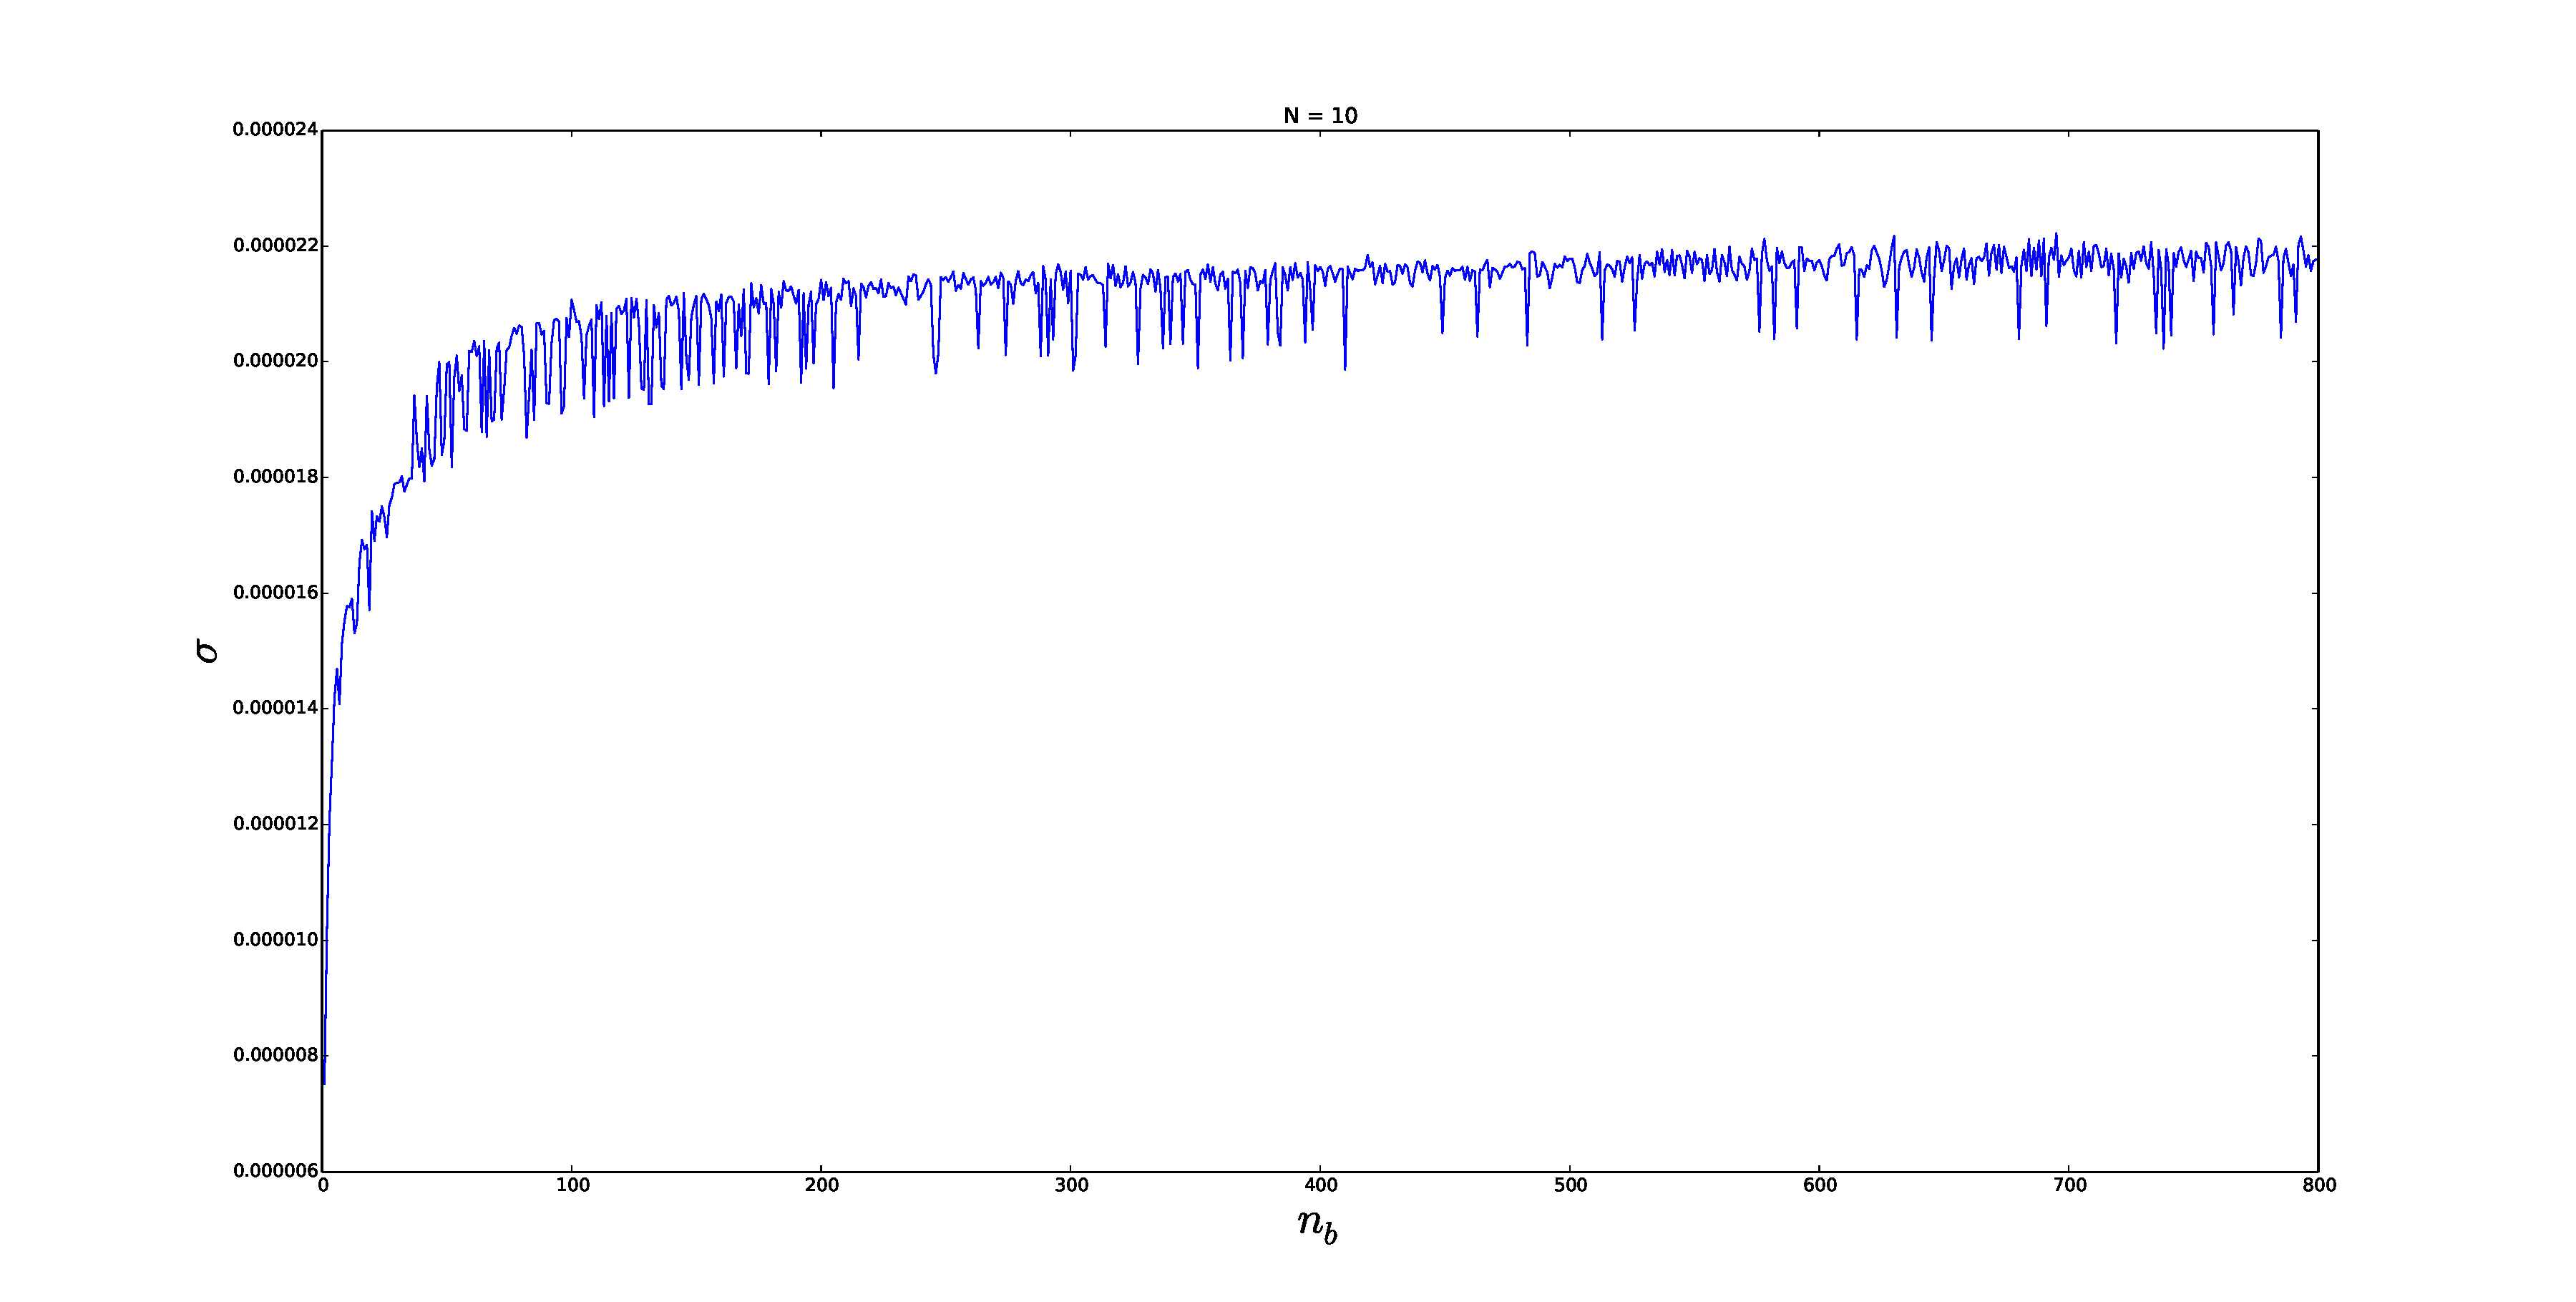
\includegraphics[width = 160mm]{error_10.pdf}
  \caption{N = 10}\label{fig:error10}
  \end{center}
\end{figure}

\begin{figure}[H]
\begin{center}
  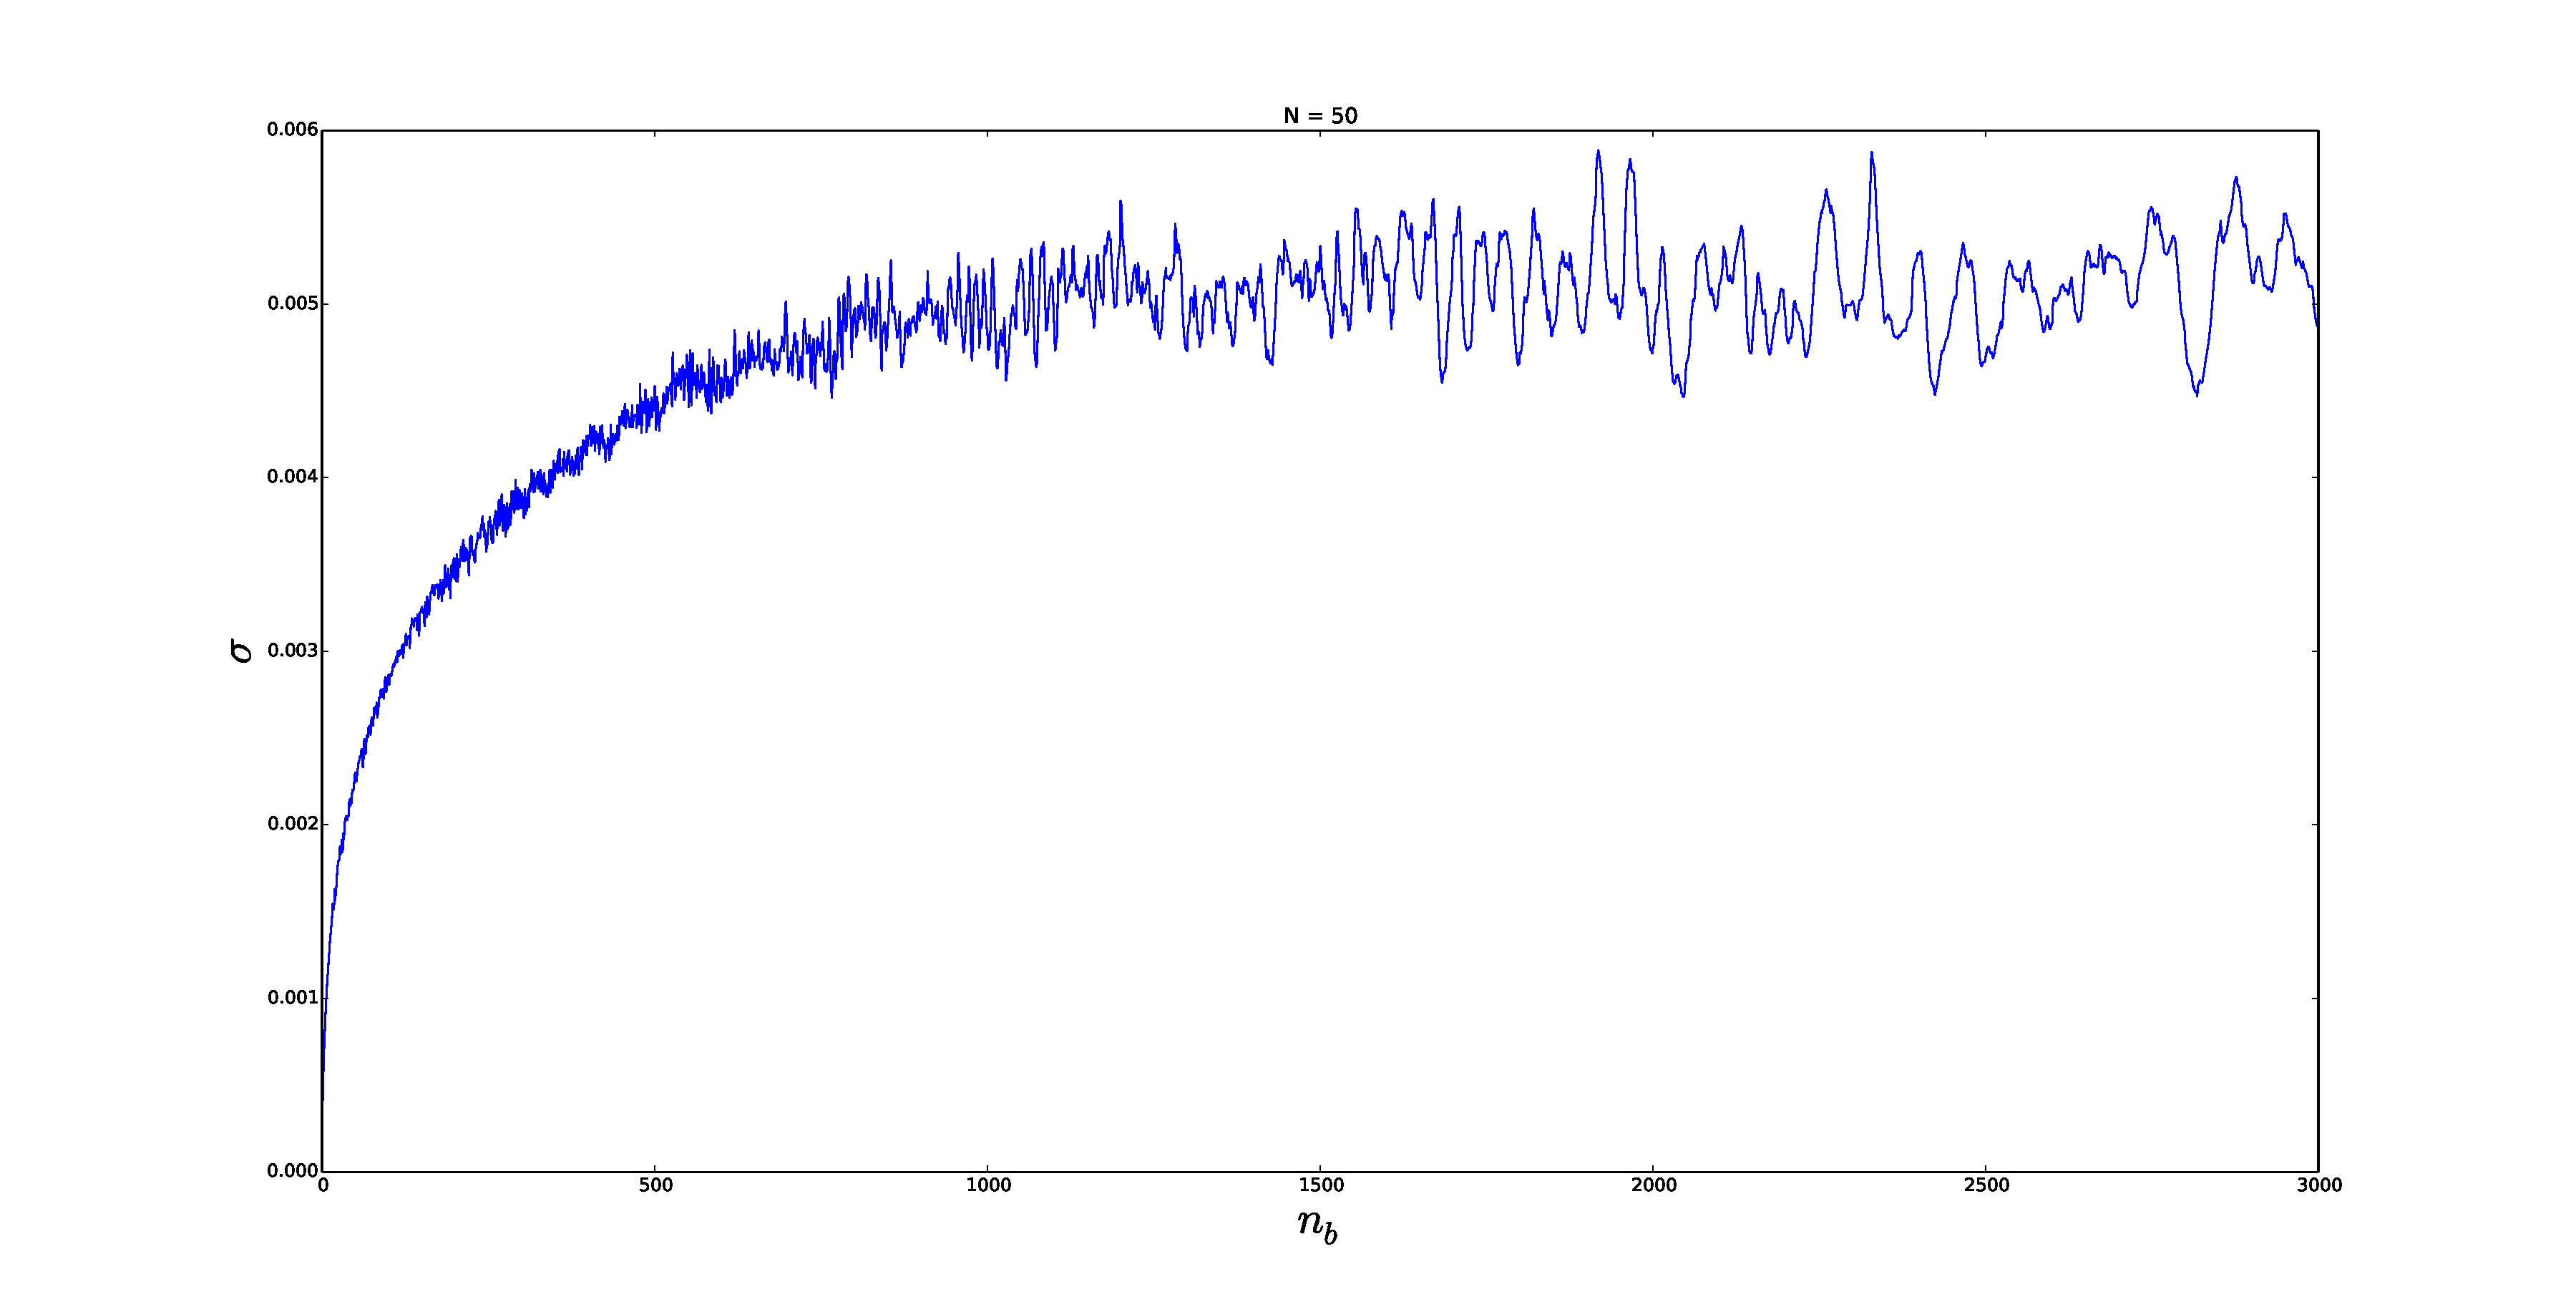
\includegraphics[width = 160mm]{error_50.pdf}
  \caption{N = 50}\label{fig:error50}
  \end{center}
\end{figure}

\begin{figure}[H]
\begin{center}
  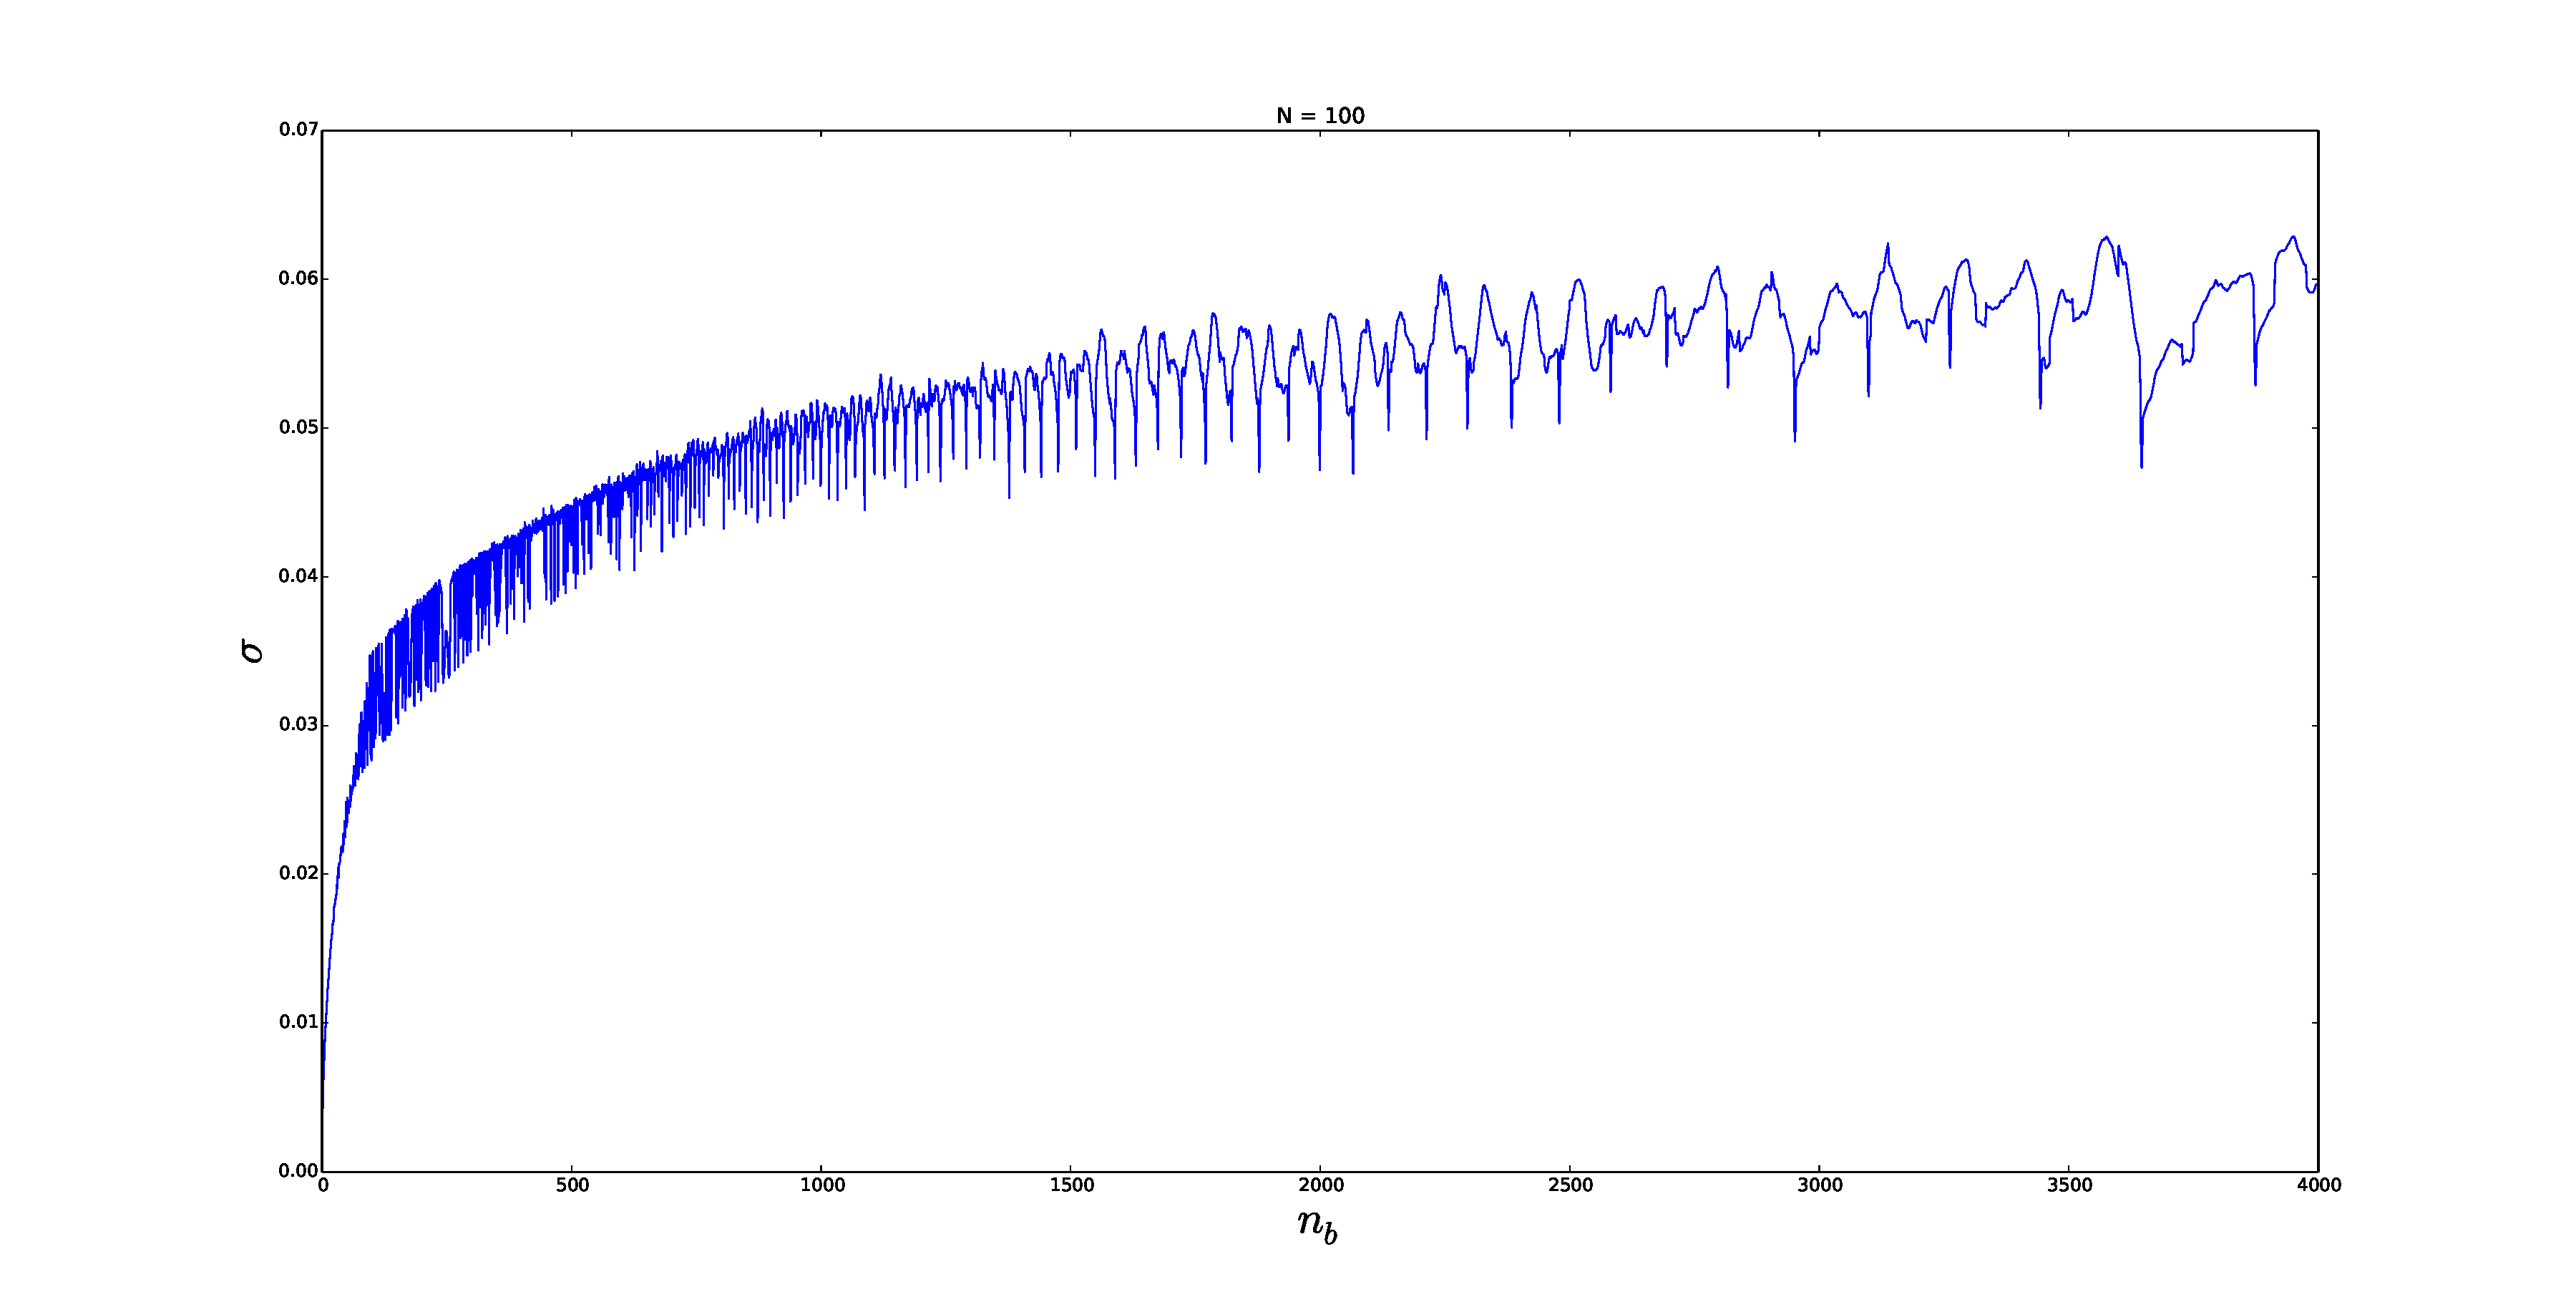
\includegraphics[width = 160mm]{error_100.pdf}
  \caption{N = 100}\label{fig:error100}
  \end{center}
\end{figure}
We can now estimate $\tau$ by looking at which block size $n_b$ the plateau is reached and multiply
this value with the above Monte Carlo step size, 
\begin{itemize}
 \item N=10: $n_b \approx 100 \Rightarrow \tau = 100\cdot 1.5 = 150$ 
 \item N=50: $n_b \approx 1000 \Rightarrow \tau = 1000\cdot 1.5 = 1500$
 \item N=100: $n_b \approx 1500 \Rightarrow \tau = 1500\cdot 1.5 = 2250$
\end{itemize}
The true sample errors are then, according to \eqref{trueSampleError},
\begin{itemize}
 \item N=10: $\sigma_{true} = 0.032$
 \item N=50: $\sigma_{true} = 0.77$
 \item N=100: $\sigma_{true} = 6.1$
\end{itemize}
We observe that the true sample errors are almost one order of magnitude larger than the uncorrelated
error estimates. 


\subsection{One-body density}
The one-body density is defined as
\begin{equation}
 \rho({\bf r}) = \int d{\bf r}_2 \dots d{\bf r}_N |\Psi({\bf r}, {\bf r}_2, \dots , {\bf r}_N)|^2
\end{equation}
This quantity can be visuzalized by making a histogram of the radial distance of the bosons.
The following paramters,
\belowcaptionskip=-10pt
\begin{lstlisting}[label=parameters3,caption=Parameters one-body density]
    int numberOfDimensions  = 3;
    int numberOfParticles   = 30;
    int numberOfSteps       = (int) 1e6;
    double omega            = 1.0;          // oscillator frequency
    double alpha            = 0.5;          // variational parameter 1
    double beta             = 2.82843;      // variational parameter 2
    double stepLength       = 1.5;          // metropolis step length
    double equilibration    = 0.1;          // amount of the total steps used
    double a                = 0.0043;       // hard sphere radius
    double gamma            = 2.82843;      // trap potential strength z-direction
\end{lstlisting}
results in
\begin{figure}[H]
\begin{center}
  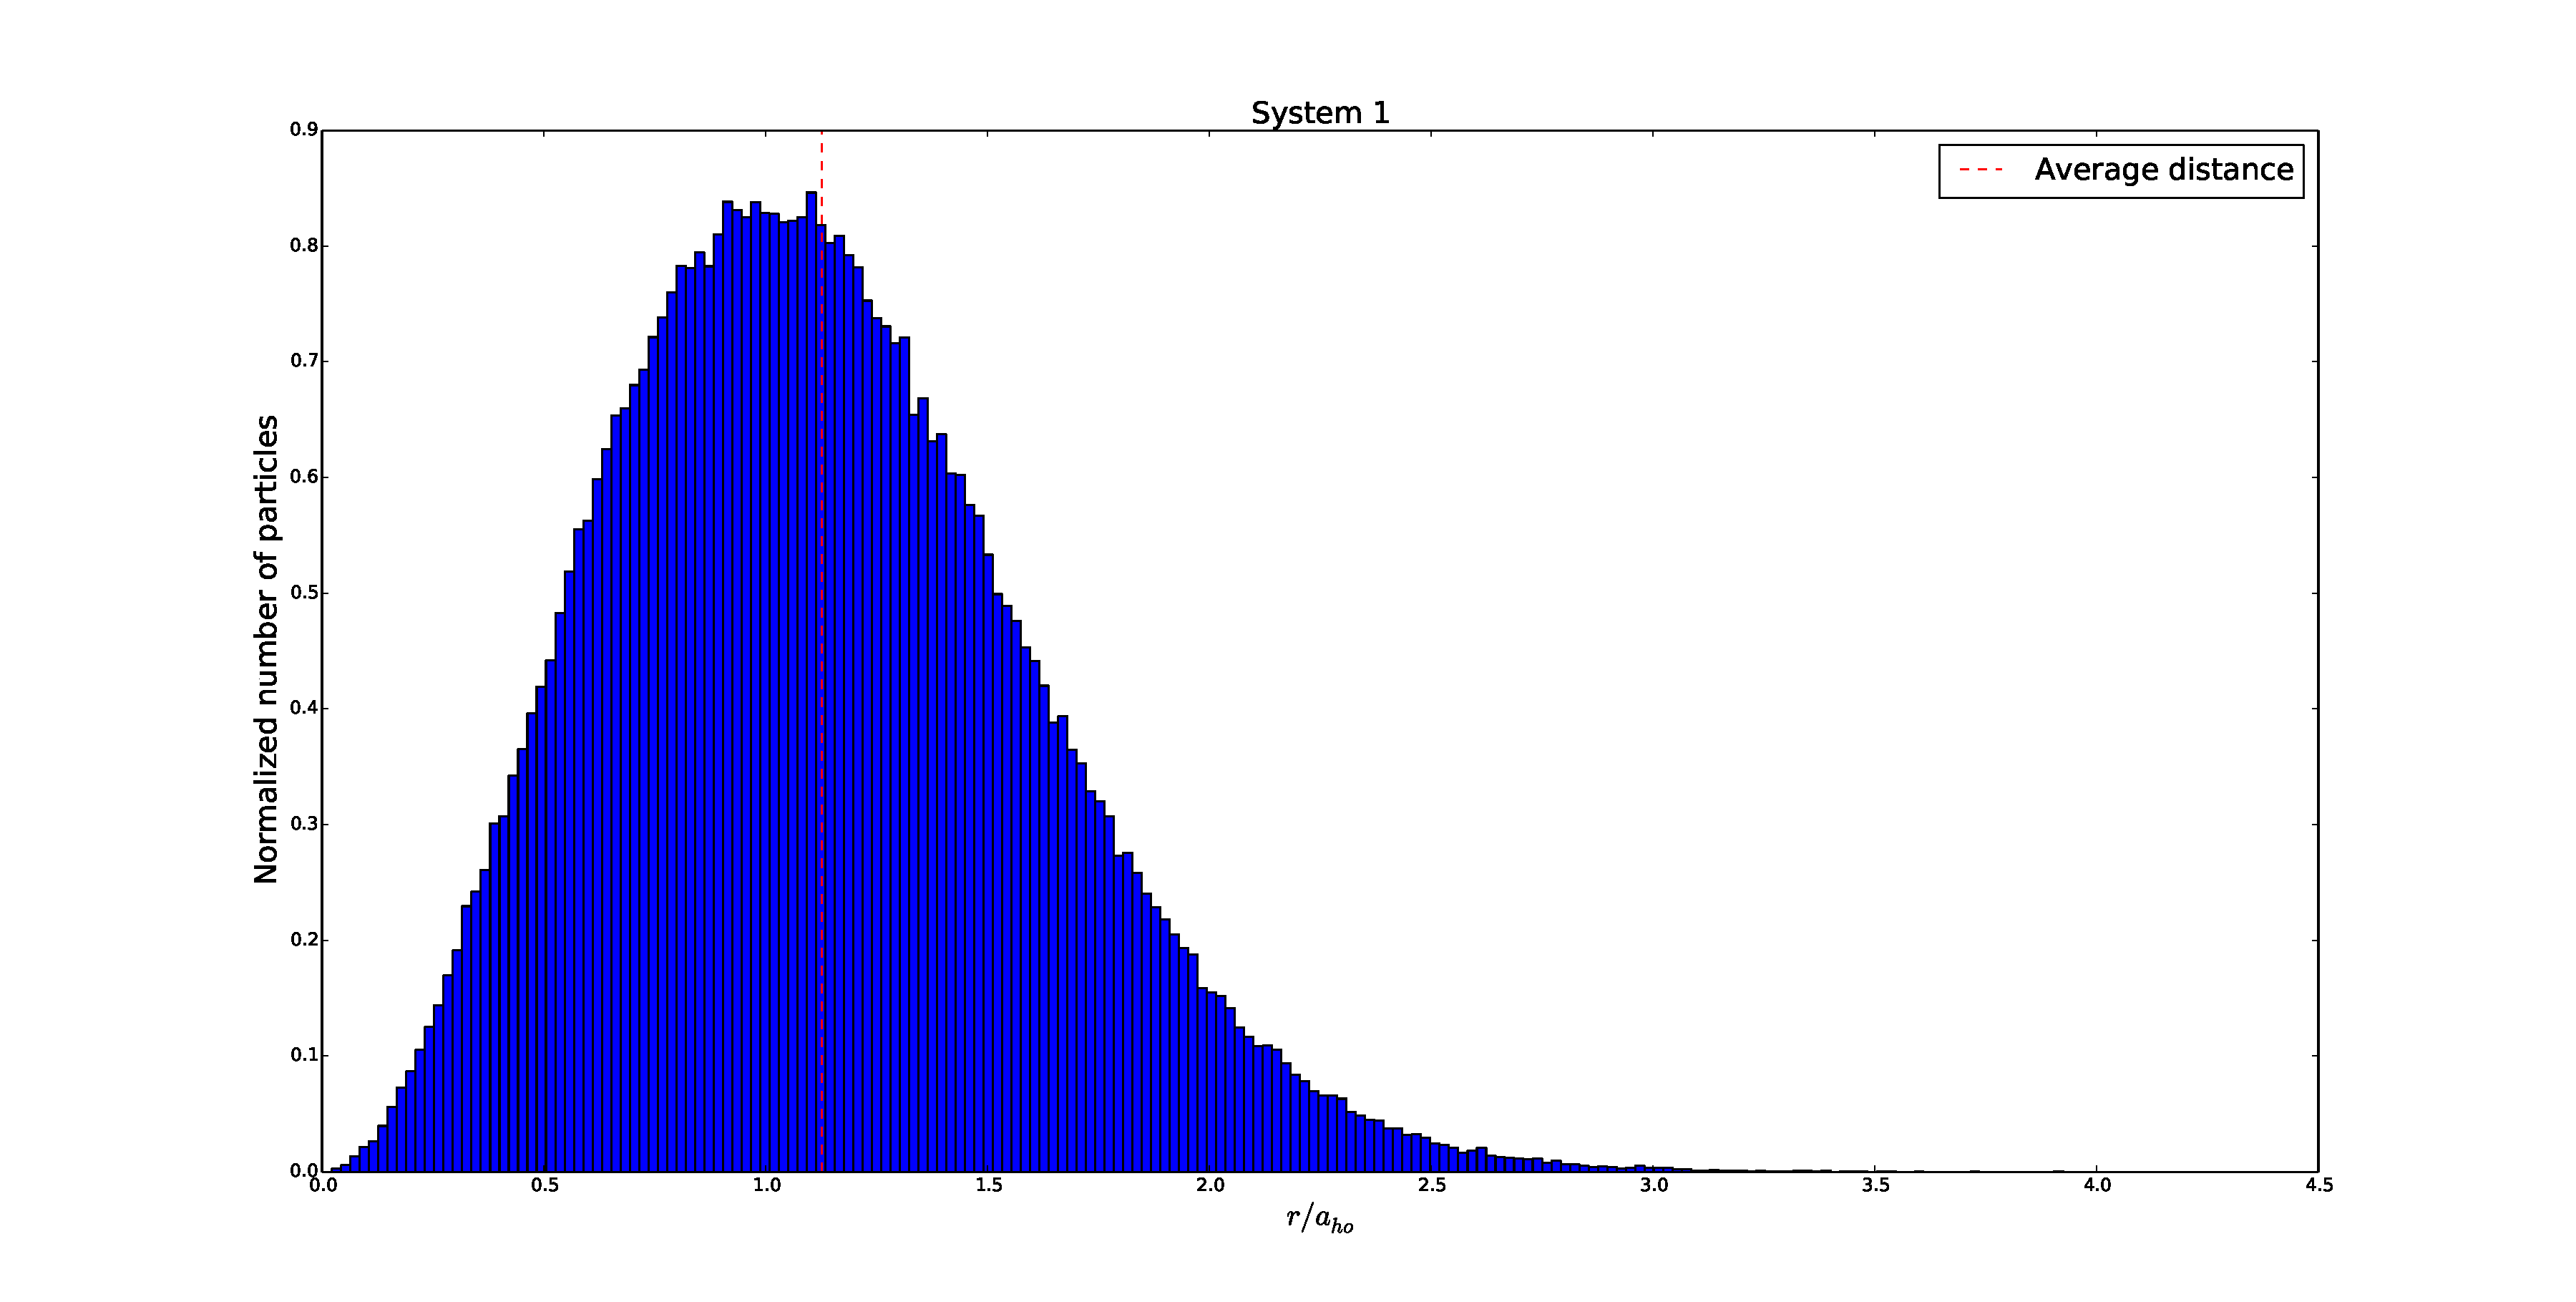
\includegraphics[width = 200mm]{radialDistSystem1.pdf}
  \caption{Radial distribution of particles - system 1}\label{fig:density1}
  \end{center}
\end{figure}

\begin{figure}[H]
\begin{center}
  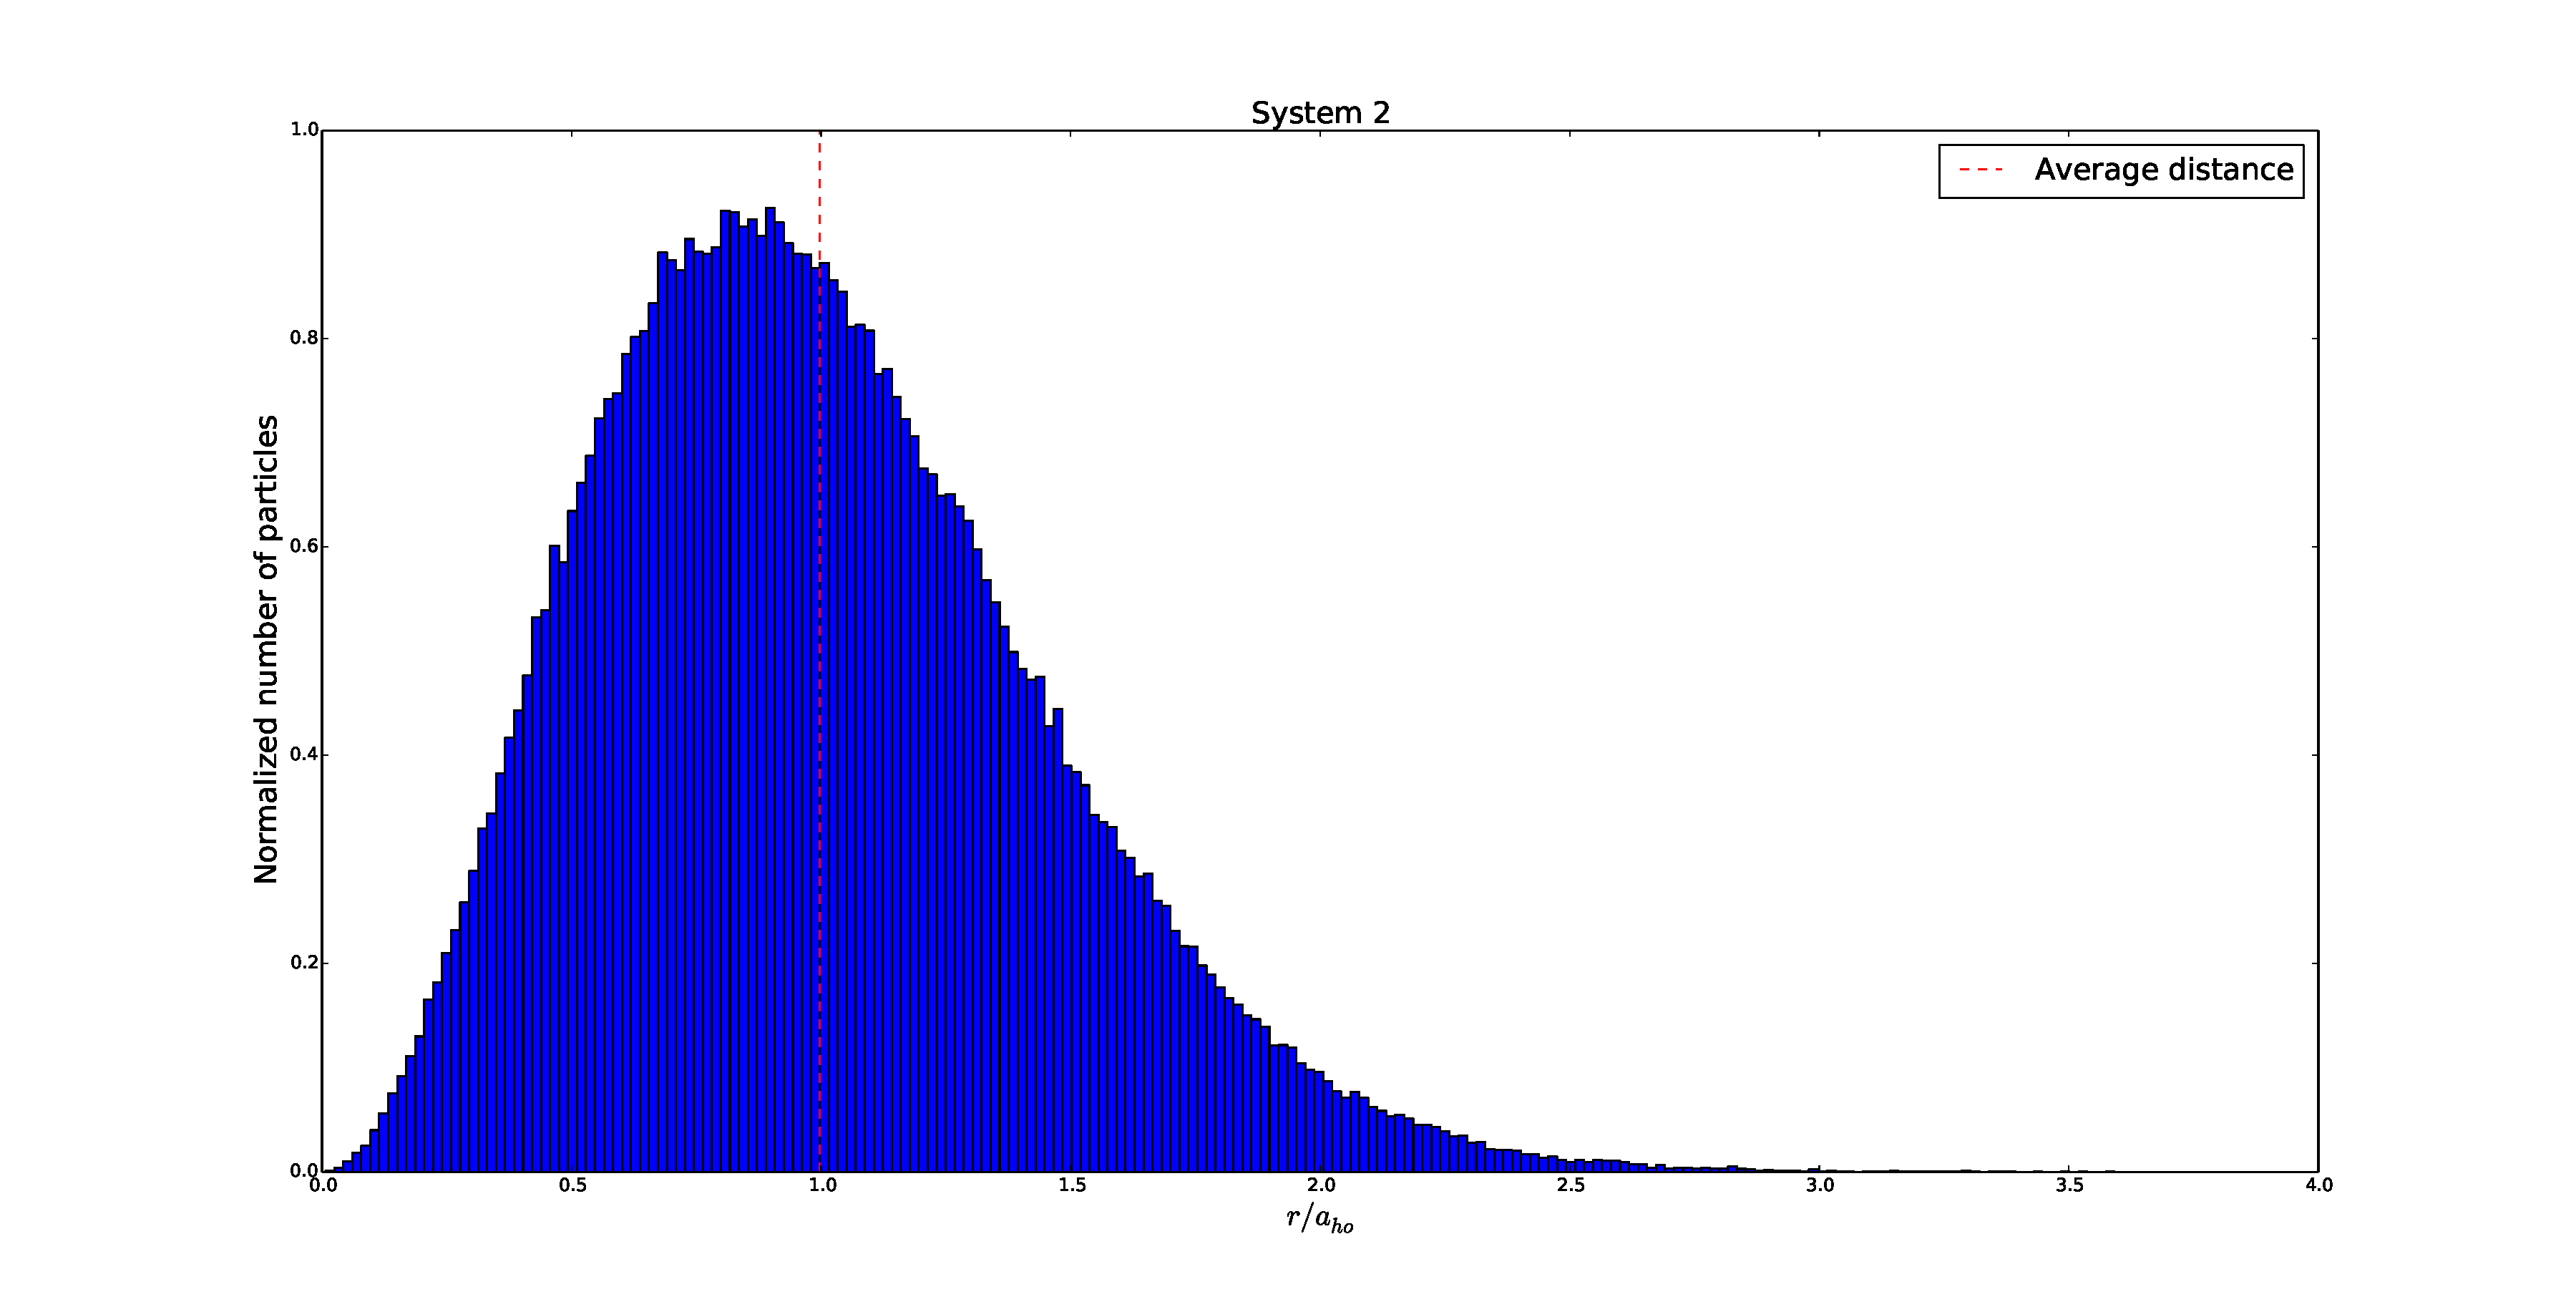
\includegraphics[width = 200mm]{radialDistSystem2.pdf}
  \caption{Radial distribution of particles - system 2}\label{fig:density2}
  \end{center}
\end{figure}
The distribution for system 1 is shifted towards the right compared to system 2, thus
the average radial distance is larger. \\

\noindent The distribution of particles in the $yz$-plane is included for visualization purposes,
\begin{figure}[H]
\begin{center}
  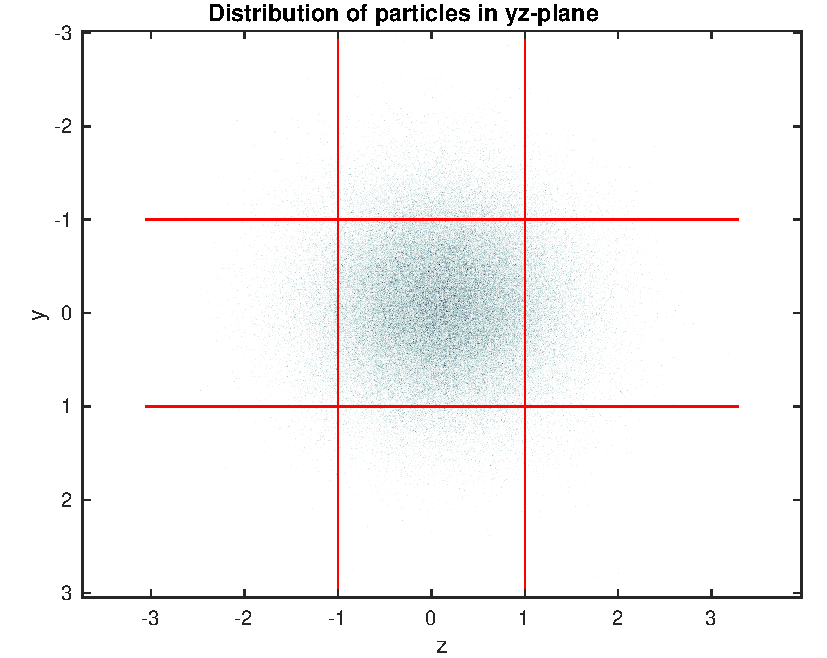
\includegraphics[width = 140mm]{radialDist1YZ.pdf}
  \caption{System 1}\label{fig:density3}
  \end{center}
\end{figure}

\begin{figure}[H]
\begin{center}
  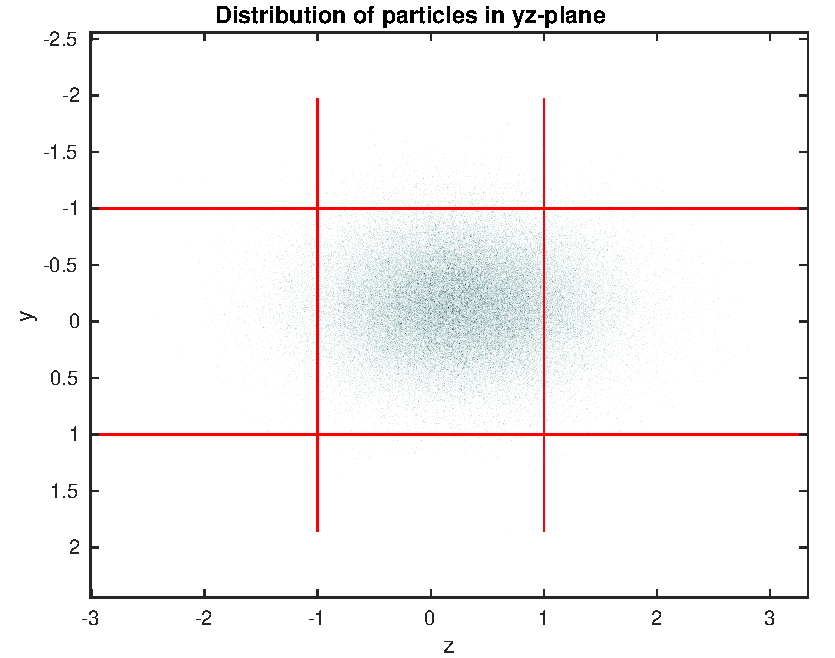
\includegraphics[width = 140mm]{radialDist2YZ.pdf}
  \caption{System 2}\label{fig:density4}
  \end{center}
\end{figure}
We observe also here that system 1 is more spread out than system 2. System 1 has a spherical distribution
centered around origo. System 2 is however shifted towards positive y- and z-direction and has a slightly 
elliptical shape with an elongation in the z-direction. 
The latter is caused by the elliptical harmonic oscillator potential \eqref{trap_eqn} with
$\omega_z / \omega_{ho} = 2.82834$.


\section{Conclusions}

For system 1, the exact ground state energies were reproduced with zero error when using the closed-form expression
for the Laplacian of the wave function. Computing this quantity numerically resulted in a small variance caused by 
the error in the differentiation algorithm. Implementing closed-form expressions saved significant CPU time. 

The error in the energies for system 2 were larger, but quite close to those in \cite{ref1}. This tells us 
that the optimal $\alpha$ found by the steepest descent method was a good approximation. 
Doing a proper error analysis by applying the blocking method was important to estimate the true sample errors, which was
almost one order of magnitude larger than the initial suggestions. 

The one-body density visualizations showed that system 2 were more dense than system 1. The different traps we used
decided how the distribution of particles looked like: The spherical trap resulted in a spherical distribution
centered around zero, while the elliptical trap stretched out the distribution in the z-direction. 

The framework we have developed can also be used to model fermionic systems if we include the proper
symmetry requirements. Further optimization of the code can be done, especially by applying parallelization. 




\section{Appendix}

\subsection{Closed-form expressions}

The quantity we are aiming to compute is the expectiation value of the so-called local energy
 \begin{equation}
    E_L({\bf R})=\frac{1}{\Psi_T({\bf R})}H\Psi_T({\bf R}),
    \label{localenergy2}
 \end{equation}
We can find closed-form expressions for the local energy with our specific Hamiltonian $H$ and trial wavefunction $\Psi_T$.
Computing the local energy involves a second derivative of $\Psi_T$, which can be expensive to compute numerically. 
Analytical expressions are therefore useful, as they can speed up the computations.\\

\noindent First, we find the local energy with only the (spherical) harmonic oscillator potential, that is we set $a=0$ and $\beta=1$.
During these calcuations we will use natural units, thus $\hbar=m=1$.
For one particle in one dimension we have
\begin{equation}
\Psi_T(x) = e^{-\alpha x^2}
\end{equation}
and
\begin{equation}
    H =  
	 -\frac{1}{2}
	 \frac{\partial^2}{\partial x^2} +
	 \frac{1}{2}\omega x^2
\end{equation}
The second derivate of the trial wave function is
\begin{equation}
 \frac{\partial^2 \Psi_T}{\partial x^2} = 2\alpha e^{-\alpha x^2}(2\alpha x^2 - 1)
\end{equation}
so that
\begin{equation}
 E_L = \frac{1}{\Psi_T}H\Psi_T = \alpha(1 - 2\alpha x^2) + \frac{1}{2}\omega^2x^2
\end{equation}
In three dimensions the double derivative is replaced by the Laplacian when computing the kinetic energy
\begin{align}
 \frac{1}{\Psi_T}\bigtriangledown^2\Psi_T &= 2\alpha(2\alpha x^2 - 1) + 2\alpha(2\alpha y^2 - 1) + 2\alpha(2\alpha z^2 - 1) \\
                          &= 2\alpha(2\alpha r^2 - 3) \label{analytickinnoninteracing}
\end{align}
thus the local energy is
\begin{equation}
 E_L = \frac{1}{\Psi_T}\left(-\frac{1}{2}\bigtriangledown^2\Psi_T + V_{ext}\right) = \alpha(3 - 2\alpha r^2) + 
 \frac{1}{2}\omega^2r^2 
\end{equation}
We now turn our attention to $N$ particles, with the following wavefunction and Hamiltonian
\begin{align}
 &\Psi_T({\bf R}) = \prod_i e^{-\alpha r_i^2} \\ \label{wfsystem1}
 &H =     \sum_i^N \left(
	 -\frac{1}{2}
	 { \bigtriangledown }_{i}^2 +
	 \frac{1}{2}\omega^2r_i^2 \right)
\end{align}
The first term of the k-th Laplacian of this wavefunction is
\begin{equation}
 \bigtriangledown^2_k\prod_i e^{-\alpha r_i^2} = 2\alpha(2\alpha x_k^2 - 1)\prod_i e^{-\alpha r_i^2}
\end{equation}
and when we divide with $\Psi_T$ to obtain the the local energy we end up with
\begin{equation}
 E_L = \sum_i^N \left( \alpha(3 - 2\alpha r_i^2) + \frac{1}{2}\omega^2r_i^2 \right)
\end{equation}
For one dimension the expression is
\begin{equation}
 E_L = \sum_i^N \left( \alpha(1 - 2\alpha x_i^2) + \frac{1}{2}\omega^2x_i^2 \right)
\end{equation} \\

\noindent It is also useful to compute the analytical expression for the drift force $F$ to be used in importance sampling
\begin{equation}
 F = \frac{2\nabla \Psi_T}{\Psi_T}.
\end{equation}
The gradient of $\Psi_T$ is
\begin{align}
 \nabla \Psi_T &= (-2\alpha x, -2\alpha y, -2\alpha z)e^{-\alpha r^2} \\
               &= -2\alpha e^{-\alpha r^2} \bf{r}
\end{align}
where ${\bf r} = (x, y, z)$.
Dividing by the wavefunction and multiplying with 2
\begin{equation}
 F = -4\alpha \bf{r}
\end{equation}


\subsection{Analytic energy for two-body quantum dot}

\begin{align}
 \Psi_T({\bf r_1}, {\bf r_2}) &= \textrm{exp}(-\alpha \omega(r_1^2 + r_2^2)/2)
 \textrm{exp}\left(\frac{a r_{12}}{1 + \beta r_{12}}\right) \\
 &= K_1K_2
\end{align}
Laplacian of this wave function:
\begin{equation}
 \nabla^2 \Psi_T({\bf r_1}, {\bf r_2}) = \frac{\partial \Psi_T}{\partial x_1^2} + 
 \frac{\partial \Psi_T}{\partial y_1^2} + \frac{\partial \Psi_T}{\partial x_2^2} +
 \frac{\partial \Psi_T}{\partial y_2^2}
\end{equation}
Using the following
\begin{equation},
 \frac{\partial r_1}{\partial x_1} = x_1/r_1
\end{equation}
and 
\begin{equation}
 \frac{\partial r_{12}}{\partial x_1} = (x_1 - x_2)/r_1
\end{equation}
Gradient of first term:
\begin{equation}
 \frac{\partial K_1}{\partial x_1} = -\alpha \omega x_1 K_1
\end{equation}
so that
\begin{equation}
 \nabla K_1 = -\alpha \omega K_1 (x_1, y_1, x_2, y_2)
\end{equation}
Gradient of second term:
\begin{equation}
 \frac{\partial K_2}{\partial x_1} = K_2 \frac{a(x_1 - x_2)}{r_{12}(1 + \beta r_{12})^2}
\end{equation}
so that
\begin{equation}
 \nabla K_2 = K_2 \frac{a}{r_{12}(1 + \beta r_{12})^2} (x_1 - x_2, y_1 - y_2, x_2 - x_1, y_2 - y_2)
\end{equation}
Laplacian of first term:
\begin{equation}
 \frac{\partial^2 K_1}{\partial x_1^2} = K_1 (\alpha^2 \omega^2 x_1^2 -\alpha \omega )  
\end{equation}
so that
\begin{equation}
 \nabla^2 K_1 = K_1 (\alpha^2 \omega^2 (r_1^2 + r_2^2) - 4\alpha \omega)
\end{equation}
Laplacian of second term:
\begin{align}
 \frac{\partial^2 K_2}{\partial x_1^2} &= K_2 \Biggr[\frac{a^2(x_1-x_2)^2}{r_{12}^2(1 + \beta r_{12})^4} +
 \frac{ar_{12}(1 + \beta r_{12})^2}{r_{12}^2(1 + \beta r_{12})^4} \\
 &-\frac{a(x_1 - x_2)[(x_1-x_2)/r_{12} (1 + \beta r_{12})^2 + 2r_{12}(1 + \beta r_{12})\beta(x_1-x_2)/r_{12}]}
 {r_{12}^2(1 + \beta r_{12})^4} \Biggr] \\
 &= K_2 \Biggr[\frac{a^2(x_1-x_2)^2}{r_{12}^2(1 + \beta r_{12})^4} +
 \frac{a}{r_{12}(1 + \beta r_{12})^2} \\
 &-\frac{a(x_1 - x_2)^2}{r_{12}^3(1 + \beta r_{12})^2}
 - \frac{2a\beta(x_1 - x_2)^2} {r_{12}^2(1 + \beta r_{12})^3} \Biggr]
\end{align}
so that
\begin{align}
 \nabla^2 K_2 &= K_2\Biggr[\frac{2a^2}{(1 + \beta r_{12})^4} + \frac{4a}{r_{12}(1 + \beta r_{12})^2}
              - \frac{2a}{r_{12}(1 + \beta r_{12})^2} - \frac{2a\beta}{(1 + \beta r_{12})^3} \Biggr] \\
              &= K_2\frac{2a}{(1+\beta r_{12})^2}\Biggr[ \frac{a}{(1+\beta r_{12})^2} + 
              \frac{1}{r_{12}} - \frac{2\beta}{1 + \beta r_{12}} \Biggr]
\end{align}
Have that
\begin{equation}
 \nabla^2 \Psi_T = \nabla^2K_1K_2 + 2\nabla K_1\nabla K_2 + K_1\nabla^2K_2
\end{equation}
and
\begin{align}
 \nabla K_1 \nabla K_2 &= -K_1K_2 \frac{a\alpha \omega}{r_{12}(1+\beta r_{12})^2}
 \Bigr[x_1(x_1 - x_2) + y_1(y_1 - y_2) - x_2(x_1 - x_2) - y_2(y_1 - y_2)\Bigr] \\
 &= -K_1K_2 \frac{a\alpha \omega}{r_{12}(1+\beta r_{12})^2}
 \Bigr[(x_1 - x_2)(x_1 - x_2) + (y_1 - y_2)(y_1 - y_2)\Bigr] \\
 &= -K_1K_2 \frac{a\alpha \omega r_{12}}{(1+\beta r_{12})^2}
\end{align}
The analytic expression for the local energy is thus
\begin{align}
 E_L = \frac{\nabla^2\Psi_T}{\Psi_T} &= 2\alpha^2 \omega^2(r_1^2 + r_2^2) - 4\alpha \omega
 - \frac{2a\alpha \omega r_{12}}{(1+\beta r_{12})^2} \\
 &+ \frac{2a}{(1+\beta r_{12})^2}\Biggr[ \frac{a}{(1+\beta r_{12})^2} + 
              \frac{1}{r_{12}} - \frac{2\beta}{1 + \beta r_{12}} \Biggr]
\end{align}



















\begin{thebibliography}{9}

%\bibitem{ref1}
%  J. K. Nilsen, J. Mur-Petit, M. Guilleumas, M. Hjorth-Jensen and A. Polls, 
% \textit{Vortices in atomic Bose-Einstein condensates in the large-gas-parameter region}, 
%  Phys. Rev. A {\bf 71}, 053610 (2005).

\bibitem{ref1}
 M. Taut, 
 \textit{Two electrons in an external oscillator potential: Particular analytic solutions
 of a Coulomb interaction problem}
 Phys. Rev. A {\bf 48}, 3561 - 3566 (1993).
 
 \bibitem{ref2}
 M. .L. Pedersen, G. Hagen, M. Hjorth-Jensen, S. Kvaal, and F. Pederiva, 
 \textit{Ab inito computation of the energies of circular quantum dots}
 Phys. Rev. B {\bf 84}, 115302 (2011)


\end{thebibliography}

\end{document}

\begin{comment}

% deloppgave
\begin{enumerate}
\item[\bf a)]
\item[\bf b)]
\item[\bf c)]
\item[\bf d)]
\end{enumerate}

%%%%%%%%
% Tabell
\begin{table}[H]
  \centering
  \begin{tabular}{ | c | r | r | r | r | r |}
    \hline
    & & & & & \\*
    \hline
    & & & & & \\*
    \hline
  \end{tabular}
  \caption{some caption}
  \label{tab:Tabell1}
\end{table}

%%%%%%%%
% Enkel figur
\begin{figure}[H]
\begin{center}
  \includegraphics[width = 120mm]{/users/filiphl/Desktop/Studie/Emne/ObligX/filnavn.png}
  \caption{some caption}\label{fig:fig1}
  \end{center}
\end{figure}

%%%%%%%%
% 2 figurer sbs
\begin{figure}
\begin{minipage}[t]{0.48\linewidth}
  \includegraphics[width=\textwidth]{fil}
  \caption{}
  \label{fig:minipage1}
\end{minipage}
\quad
\begin{minipage}[t]{0.48\linewidth}
\includegraphics[width=\textwidth]{fil}
  \caption{}
  \label{fig:minipage1}
\end{minipage}
\end{figure}

%%%%%%%%
% X antall kollonner
\begin{multicols*}{X}
\begin{spacing}{0.7} % verticale mellomrom
%kan f.eks benytte align?
\end{spacing}
\end{multicols*}


%%%%%%%%
%Matrise
\begin{equation*}
    {\bf A} = \left(\begin{array}{cccccc}
                           z &z &z &z &z &z \\
                           z &z &z &z &z &z \\
                           z &z &z &z &z &z \\
                           z &z &z &z &z &z \\
                           z &z &z &z &z &z \\
                           z &z &z &z &z &z \\
                      \end{array} \right)
\end{equation*}
%%%%%%%%

